\chapter{Results}

\section{Historic Range of Variability}

\subsection{Disturbance Regime}

This report focuses on the effects of wildfire as a natural disturbance; the impacts of other natural disturbances during the reference period were likely localized in time or space and therefore probably had far less impact on vegetation patterns over broad spatial and temporal scales than did fire.\todo{is this true?} In the sections below, we briefly describe the simulated disturbance regime (i.e., spatial extent and distribution, frequency and temporal variability). In this subsection, we refrain from describing variations among vegetation types - this will be accomplished in Subsection~\ref{subsec:HRVvegresponse}\todo{verify this}. Finally, it is important to realize that while the information below is presented as ``results,'' it could have easily been presented in the methods section as ``model calibration.'' Key spatial and temporal aspects of the disturbance regime were evaluated during preliminary calibration runs, and we subsequently adjusted model parameters to effect desired changes. Thus, while the information presented below does in fact represent results (output) of the simulation, it also represents a set of targets used to calibrate the model (i.e., adjust model parameters to achieve desired results). While this may seem a bit circular, it was a necessary process for a complex model such as \textsc{RMLands}. Moreover, our real emphasis was on quantifying the vegetation patterns and dynamics resulting from these disturbance processes.

\paragraph{Disturbed Area}

% 174830 eligible hectares
% 181550 hectares in core
% check math using Wildfire_darea_trajectory.csv
Approximately 96\% of the landscape was eligible for wildfire disturbance (all cover types except Barren and Water). As expected, the frequency and extent of simulated wildfires varied across timesteps (Figures~\ref{fig:darea} and~\ref{fig:darea_hist}). Remarkably, given the rotation interval and percent mortality expected over time on this landscape, large proportions of the project area burned each (5-year) timestep. On average, at least 10\% of the landscape burned at some combination of low and high mortality every ten years. Timesteps with area burned of 30\% or less were the most frequently observed. Fires covering at least 25\% of the landscape burned approximately every 25 years, and half or more of the landscape burned at a 200 year interval\todo{how did I calculate this?}. The smallest area disturbed over the course of the simulation was 0.26\%, while the largest was 66.2\% (of which 22.91\% was high mortality). In general, within a given timestep about a third of the disturbed area burned as high mortality (Table~\ref{tab:darea}. High mortality fires do include the burning of early development vegetation, including chaparral.

\begin{table}[!htbp]
\centering
\caption{Summary statistics for area disturbed by wildfire during the simulation. Values are expressed as percentage of the landscape eligible for disturbance that was actually disturbed.}
\label{tab:darea}
\begin{tabular}{@{}llll@{}}
\toprule
\textbf{\begin{tabular}[c]{@{}l@{}}Summary Statistic \\ (disturbed area/timestep)\end{tabular}}    & \textbf{Low Mortality}   & \textbf{High Mortality}    & \textbf{Any Mortality}   \\
\midrule
Minimum darea/timestep        &    0.22             & 0.03                  &     0.26            \\
Maximum darea/timestep        &   43.27             & 22.91                 &     66.2            \\
 Median darea/timestep        &    9.24             & 3.98                  &     13.12           \\
   Mean darea/timestep        &   11.58             & 5.17                  &     16.75           \\
\bottomrule
\end{tabular}
\end{table}

%\begin{verbatim}
%     summary statistic mort.low mort.high mort.any
%minimum darea/timestep     0.22      0.03     0.26
%maximum darea/timestep    43.27     22.91     66.2
% median darea/timestep     9.24      3.98    13.12
%   mean darea/timestep    11.58      5.17    16.75
%\end{verbatim}

\begin{figure}[!htbp]
\centering
\includegraphics[width=0.9\textwidth]{/Users/mmallek/Tahoe/R/Rplots/November2014/darea.png}
\caption{Disturbance trajectory for wildfire during the simulation. The first timestep is 40 because we excluded earlier timesteps as equilibration. Dark blue values represent high mortality fire, while light blue values represent low mortality fire and are stacked on top of high mortality.}
\label{fig:darea}
\end{figure}

\begin{figure}[!htbp]
\centering
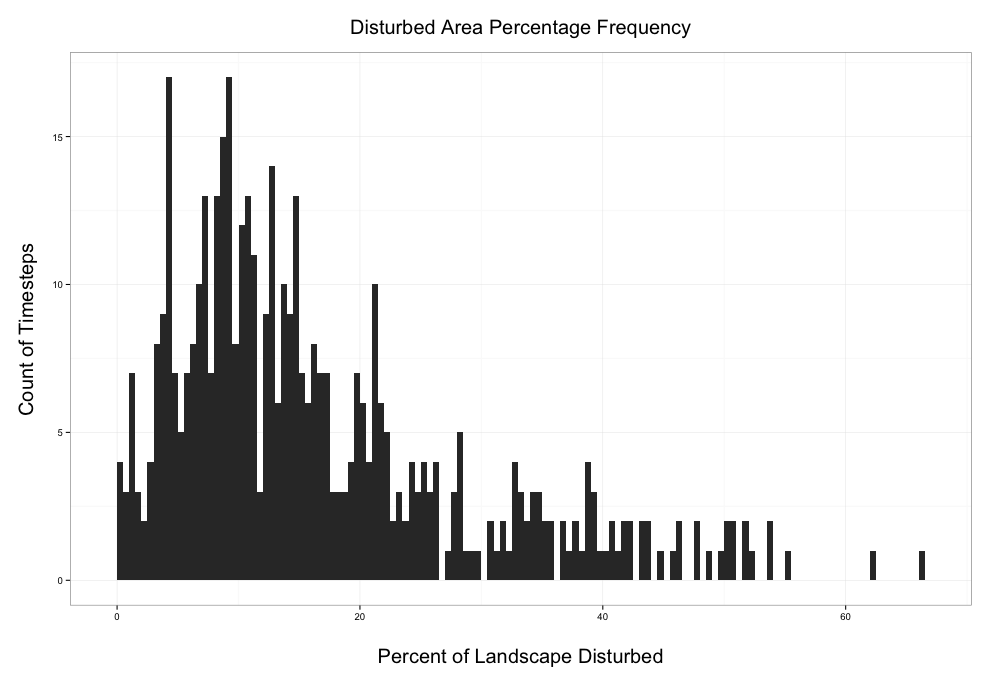
\includegraphics[width=0.6\textwidth]{/Users/mmallek/Tahoe/Report2/images/darea_hist.png}
\caption{Histogram of percent of landscape disturbed by wildfire during the simulation. The distribution is substantially right-skewed, and most fires burn less than 20\% of the eligible landscape.}
\label{fig:darea_hist}
\end{figure}



\paragraph{Disturbance Size}
As described in Section \ref{subsubsec:distparams}, we specified a target set of disturbance sizes. Because wildfire has many stochastic components, we do not expect the model results to match these targets exactly. Figure \ref{fig:dsize} compares the observed and target disturbance size distribution.

%\begin{verbatim}
%$`Wildfire disturbance size`$`run number 1`
%   bin obs.freq obs.proportion target.freq target.proportion
%     5   135327   0.7797220526        8464      0.8801996672
%    25    21339   0.1229502529         378      0.0393094842
%   125     5366   0.0309176183         316      0.0328618968
%   625     5011   0.0288721926         293      0.0304700499
%  3125     4803   0.0276737460         111      0.0115432612
% 15625     1503   0.0086599292          48      0.0049916805
% 78125      130   0.0007490291           6      0.0006239601
%133828       79   0.0004551792           0      0.0000000000
%\end{verbatim}

\begin{figure}[!htbp]
\centering
\includegraphics[width=0.7\textwidth]{/Users/mmallek/Tahoe/R/Rplots/November2014/dsize.png}
\caption{Side by side barplot of the observed and target wildfire size distribution for our 500-timestep long run of the model.}
\label{fig:dsize}
\end{figure}



\paragraph{Effect of Climate} \todo{Do I say I'll do this in methods?}Climate does have a positive relationship with disturbed area, as expected (Figure \ref{fig:climate_darea}. We show here a fitted line, but note the heteroskedastic variance about the mean. The relationship is fairly weak. During wetter-than-average years, we see less disturbed area. Over 20\% of the landscape burned only in timesteps during which the climate parameter was at least 0.75. However, over 50\% of the landscape burned in a few timesteps less than the average value, 1. Overall we observe that as climate shifts from wet to drought, the disturbed area increases. Climate also has a weak effect on the size of individual fires (Figure \ref{fig:climate_dsize}). Fire size is also influenced by vegetation susceptibility and the specified disturbance size distribution. Figure \ref{fig:compare_clim_darea} illustrates the climate parameter values and disturbed area proportion of the landscape for a subset of timesteps during the simulation.

\begin{figure}[!htbp]
  \centering
  \subfloat[][]{
    \centering
    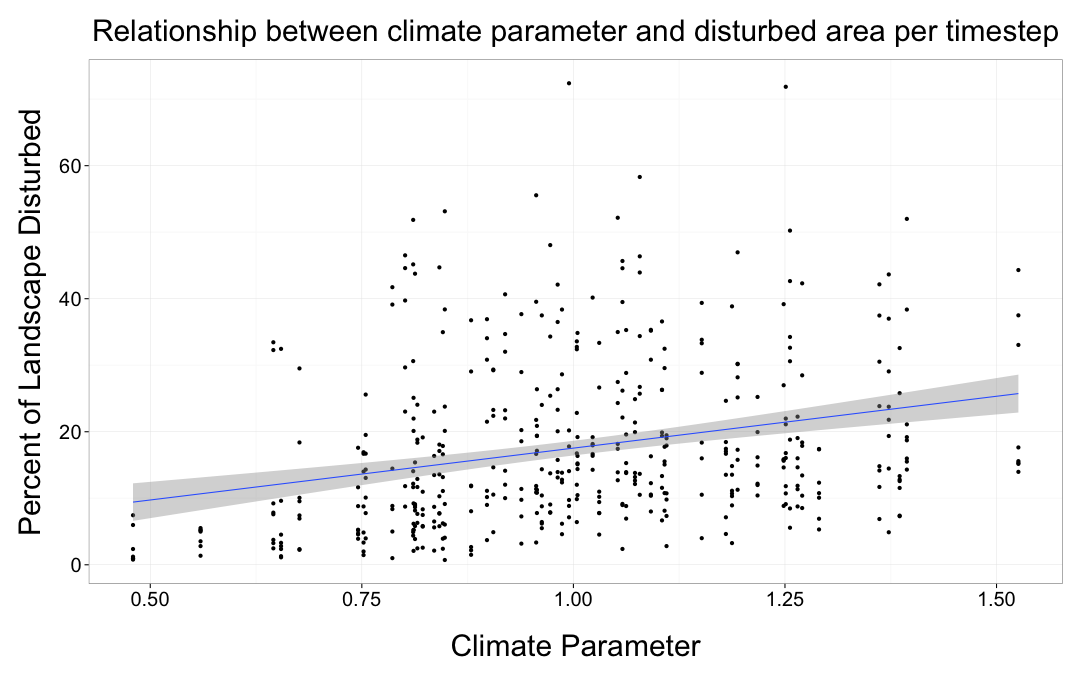
\includegraphics[width=0.5\textwidth]{/Users/mmallek/Tahoe/Report2/images/climate_darea.png}
    \label{fig:climate_darea}
  }%
  %\qquad
  \subfloat[][]{
    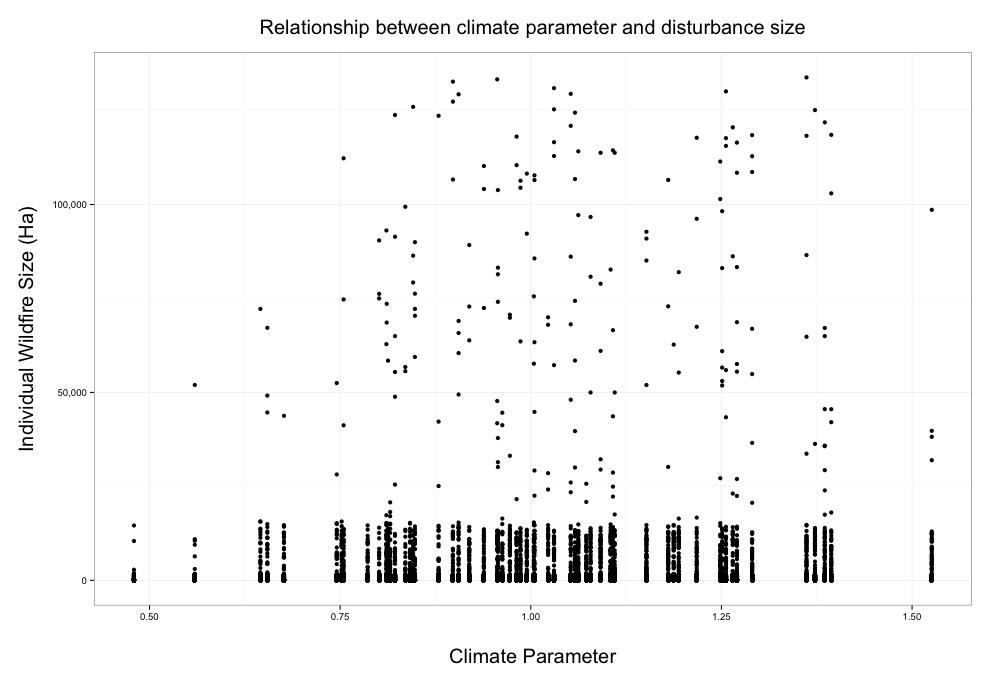
\includegraphics[width=0.5\textwidth]{/Users/mmallek/Tahoe/Report2/images/climate_dsize.png}
    \label{fig:climate_dsize}
  }
  \caption{(a) Plot of the climate parameter and disturbed area value for each timestep of the simulation (excluding the  equilibration period). A linear model has been fit to the data and is shown as a blue line; the grey shaded area represents  the 95\% confidence interval around the mean. (b) Plot showing the size of each individual wildfire and the climate parameter value in effect at the time of disturbance for each disturbance during the simulation (excluding the equilibration period).}
  \label{fig:climate_disturbance}
\end{figure}

\begin{figure}[!htbp]
\centering
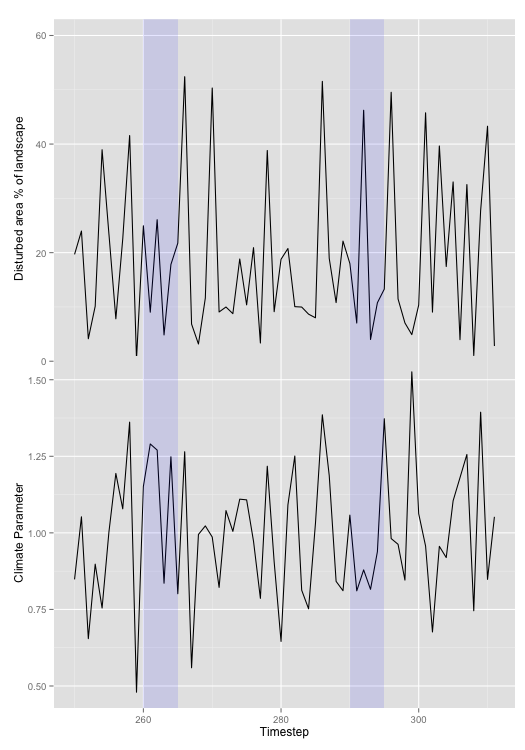
\includegraphics[width=0.8\textwidth]{/Users/mmallek/Tahoe/Report2/images/climate_darea_vert.png}
\caption{Climate parameter and proportion of eligible landscape disturbed by wildfire for timesteps 250 to 310 of the simulation.}
\label{fig:compare_clim_darea}
\end{figure}


\newpage
\paragraph{Fire Rotation}
We present here the results for non-static cover types whose extent is at least 1000 ha. Full results are presented in \todo{Appendix?}. As previously discussed, these results could have been presented in the methods section. Each of the nine cover types shown here were calibrated to within 10\% of their target values, which were based on empirical published values and local expert opinion.

\begin{table}[!htbp]
\centering
\caption{Fire rotation for the nine cover types whose extent cover at least 1000 ha.}
\begin{tabular}{@{}llll@{}}
\toprule
Land Cover Type                              & \begin{tabular}[c]{@{}l@{}}Low Mortality \\ Fire Rotation\end{tabular} & \begin{tabular}[c]{@{}l@{}}High Mortality \\ Fire Rotation\end{tabular} & \begin{tabular}[c]{@{}l@{}}All Fires \\ Rotation\end{tabular} \\ \midrule
Mixed Evergreen - Mesic                      & 63                          & 534                          & 57                 \\
Mixed Evergreen - Xeric                      & 51                          & 472                          & 46                 \\
Oak-Conifer Forest and Woodland              & 33                          & 100                          & 25                 \\
\begin{tabular}[c]{@{}l@{}}Oak-Conifer Forest and \\ Woodland -  Ultramafic\end{tabular} & 48                          & 1192                         & 46                 \\
Red Fir - Mesic                              & 101                         & 164                          & 62                 \\
Red Fir - Xeric                              & 59                          & 117                          & 39                 \\
Sierran Mixed Conifer - Mesic                & 39                          & 115                          & 29                 \\
Sierran Mixed Conifer - Ultramafic           & 106                         & 196                          & 69                 \\
Sierran Mixed Conifer - Xeric                & 40                          & 62                           & 24                 \\
Total                                        & 45                          & 100                          & 31                 \\ \bottomrule
\end{tabular}
\end{table}


\paragraph{Population Return Interval}
Overall, the point-specific return interval (grand mean) for all eligible cells ranged from 17 years to \textgreater 2500 years (cells that never burned during the simulation) for both classes of wildfire mortality (Figure \ref{fig:preturn}. The median return interval across all cover types was 42 years for low mortality fire, 111 year for high mortality fire, and 29 years for any fire. The population return interval plots and maps specific to each of the nine focal cover types follow (Figures \ref{fig:preturn_megm} through \ref{fig:preturn_smcx}.).

\begin{figure}[!htbp]
  \centering
  \subfloat[][]{
    \centering
    \includegraphics[height=0.4\textheight]{/Users/mmallek/Tahoe/R/Rplots/November2014/preturn_all.png}
    \label{fig:preturn_plot}
  }%
  \qquad
  \subfloat[][]{
    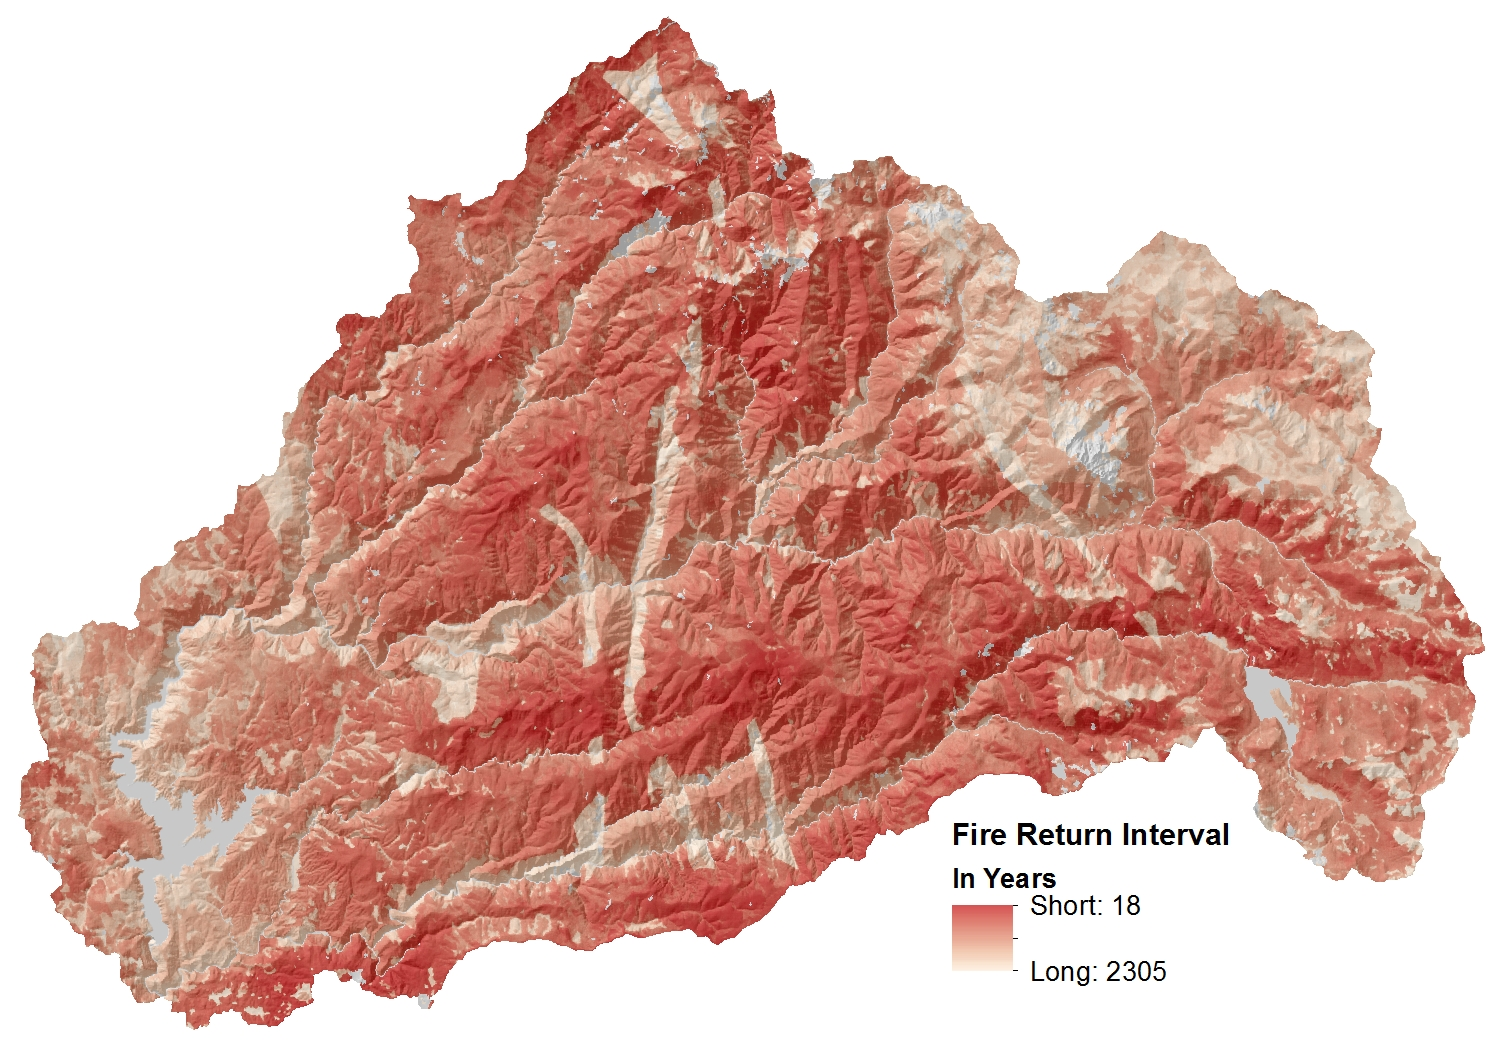
\includegraphics[height=0.4\textheight]{/Users/mmallek/Tahoe/Report2/images/fri_all.jpg}
    \label{fig:preturn_map}
  }
  \caption{(a) Population return interval (average number of years between fires) distribution for the full landscape under study. The population return interval is the point-specific interval, sometimes described as the ``grand mean'' for a given point. (b) Spatial depiction of fire return intervals across the landscape, for all cover types, in terms of fire return interval. The value at any given cell is the point-specific return interval.}
  \label{fig:preturn}
\end{figure}


\begin{figure}[!htbp]
  \centering
  \subfloat[][]{
    \centering
    \includegraphics[width=0.5\textwidth]{/Users/mmallek/Tahoe/R/Rplots/November2014/preturn_megm.png}
    }%
  \subfloat[][]{
    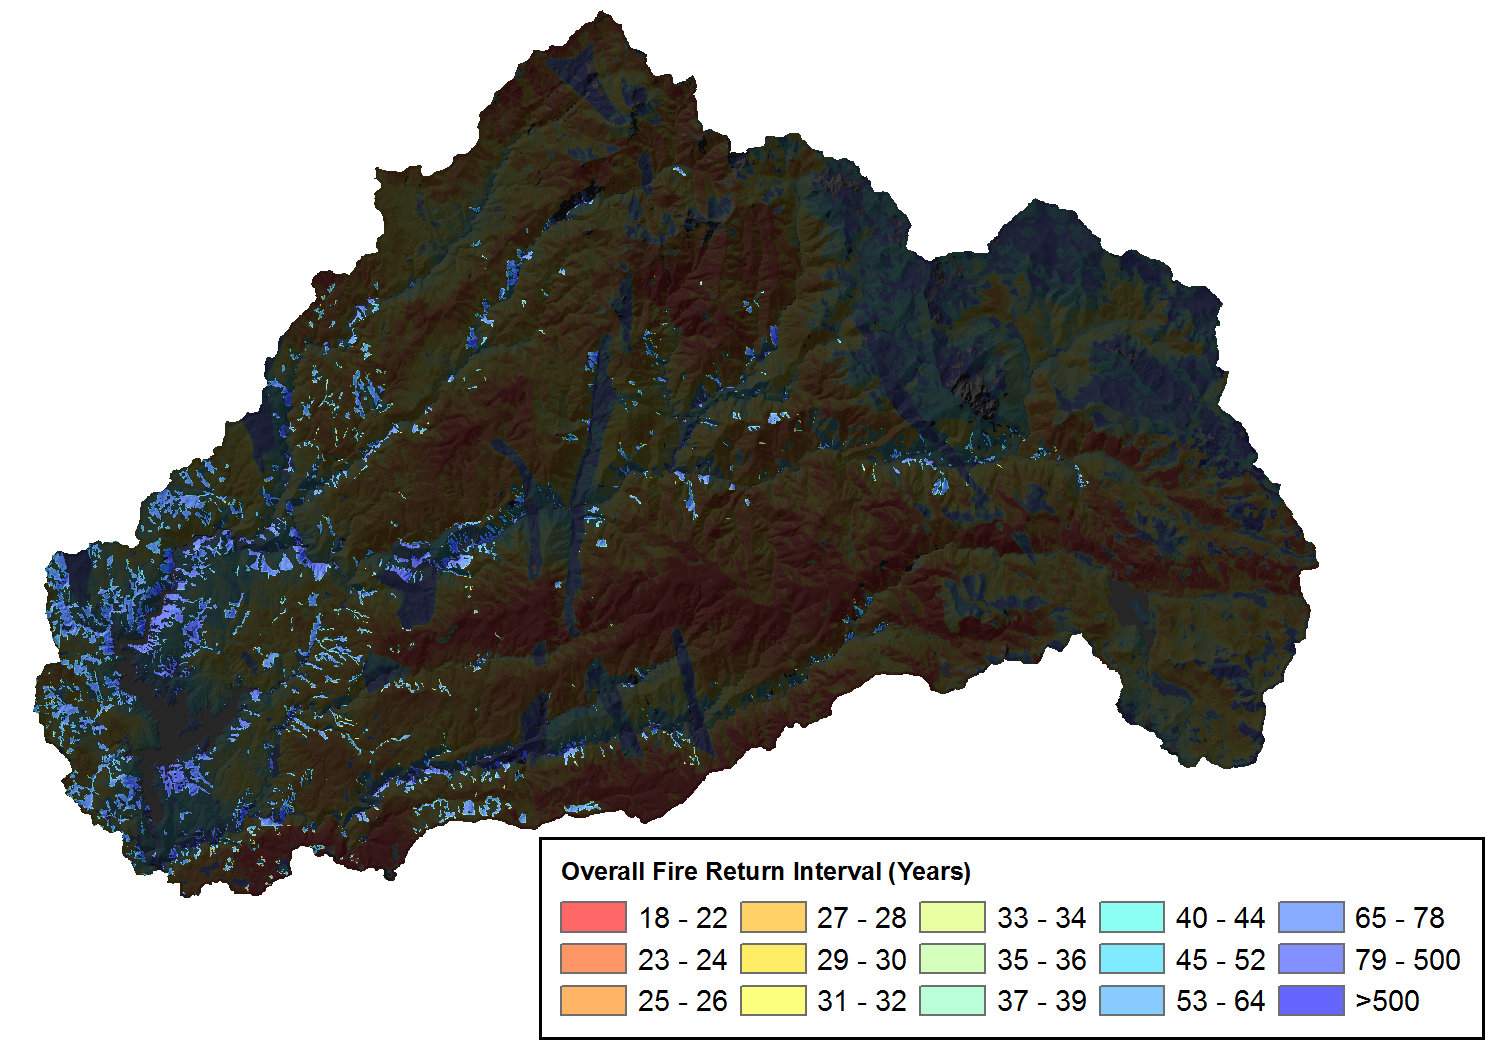
\includegraphics[width=0.5\textwidth]{/Users/mmallek/Tahoe/Report2/images/fri_megm.png}
    }
  \caption{(a) Population return interval (average number of years between fires) distribution for Mixed Evergreen - Mesic. (b) Spatial depiction of fire return intervals across the landscape. Cover types other than Mixed Evergreen - Mesic are partially obscured in grey. The value at any given cell is the point-specific return interval, which ranges from 19 years to \textgreater 1000 years.}
    \label{fig:preturn_megm}
\end{figure}

\begin{figure}[!htbp]
  \centering
  \subfloat[][]{
    \centering
    \includegraphics[width=0.5\textwidth]{/Users/mmallek/Tahoe/R/Rplots/November2014/preturn_megx.png}
    }%
  \subfloat[][]{
    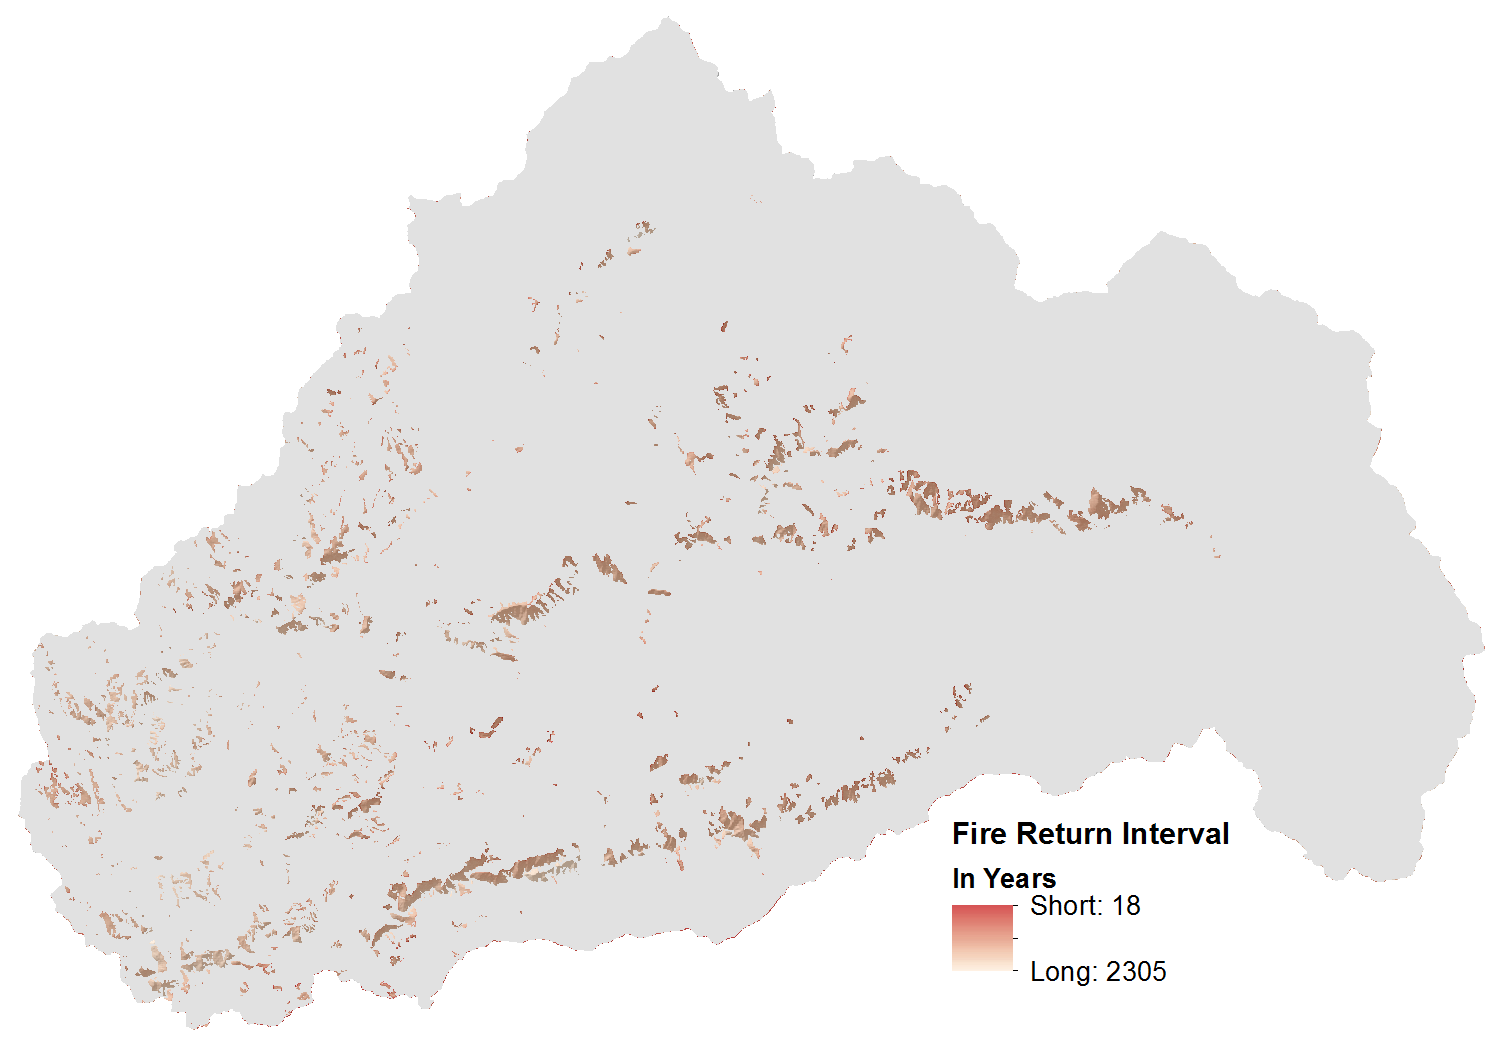
\includegraphics[width=0.5\textwidth]{/Users/mmallek/Tahoe/Report2/images/fri_megx.png}
    }
  \caption{(a) Population return interval (average number of years between fires) distribution for Mixed Evergreen - Xeric.  (b) Spatial depiction of fire return intervals across the landscape. Cover types other than Mixed Evergreen - Xeric are partially obscured in grey. The value at any given cell is the point-specific return interval, which ranges from 20 years to \textgreater 1000 years.}
\label{fig:preturn_megx}
\end{figure}

\begin{figure}[!htbp]
  \centering
  \subfloat[][]{
    \centering
    \includegraphics[width=0.5\textwidth]{/Users/mmallek/Tahoe/R/Rplots/November2014/preturn_ocfw.png}
    }%
  \subfloat[][]{
    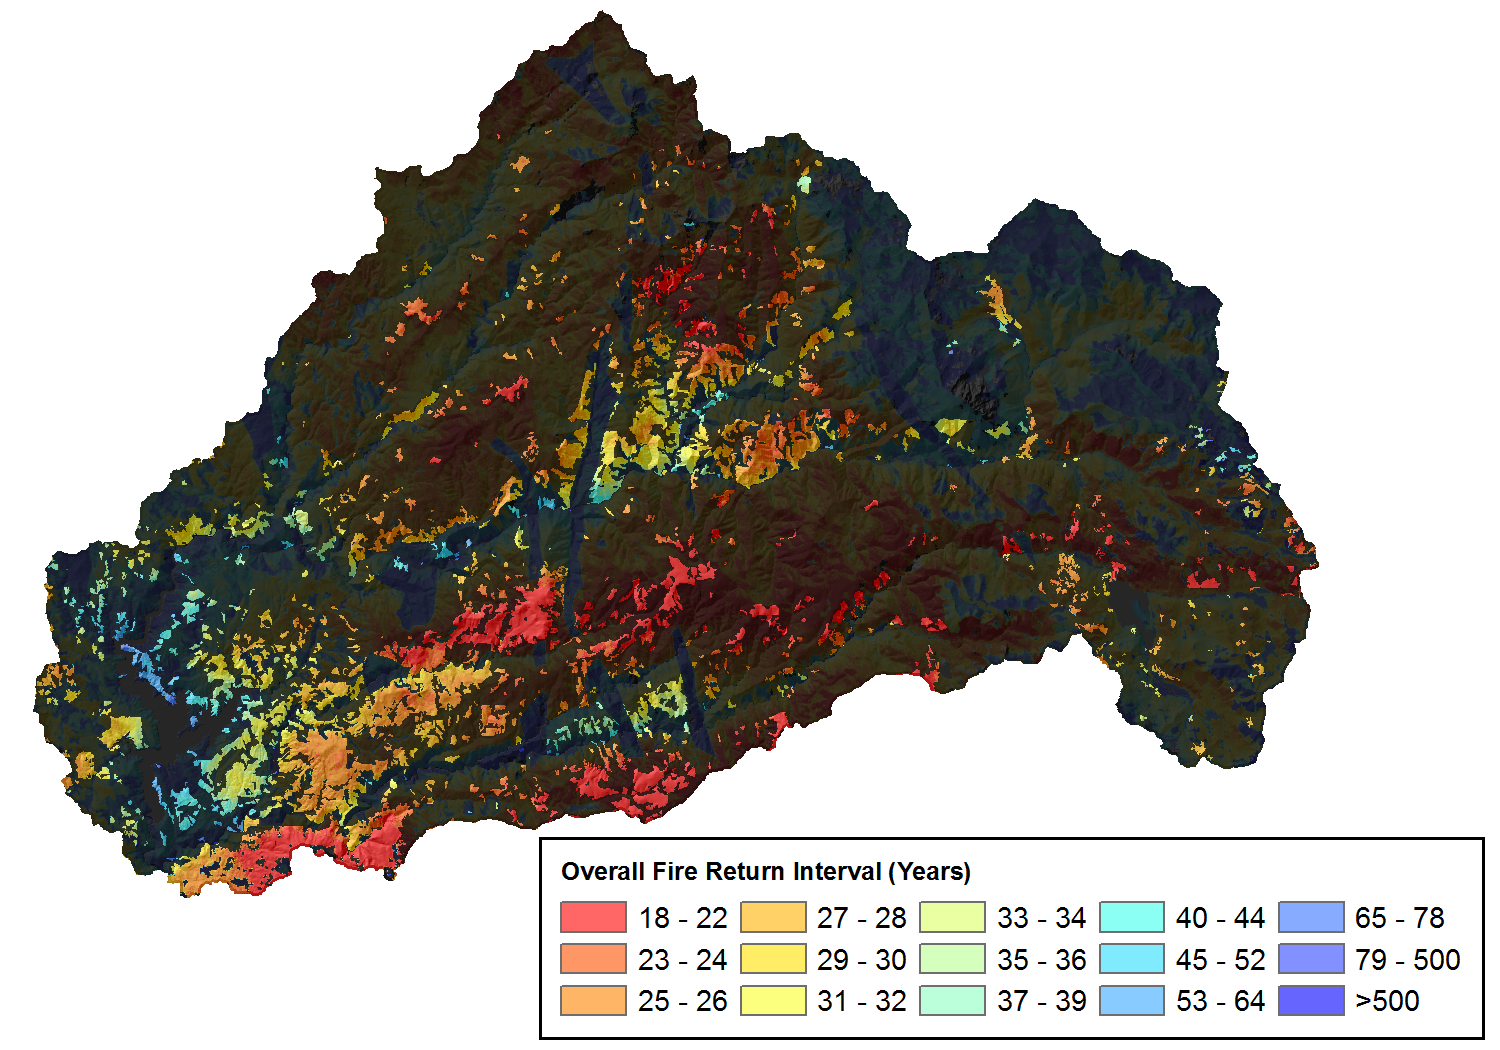
\includegraphics[width=0.5\textwidth]{/Users/mmallek/Tahoe/Report2/images/fri_ocfw.png}
    }
  \caption{(a) Population return interval (average number of years between fires) distribution for Oak-Conifer Forest and Woodland.  (b) Spatial depiction of fire return intervals across the landscape. Cover types other than Oak-Conifer Forest and Woodland are partially obscured in grey. The value at any given cell is the point-specific return interval, which ranges from 17 years to \textgreater 1000 years.}
\label{fig:preturn_ocfw}
\end{figure}

\begin{figure}[!htbp]
  \centering
  \subfloat[][]{
    \centering
    \includegraphics[width=0.5\textwidth]{/Users/mmallek/Tahoe/R/Rplots/November2014/preturn_ocfwu.png}
    }%
  \subfloat[][]{
    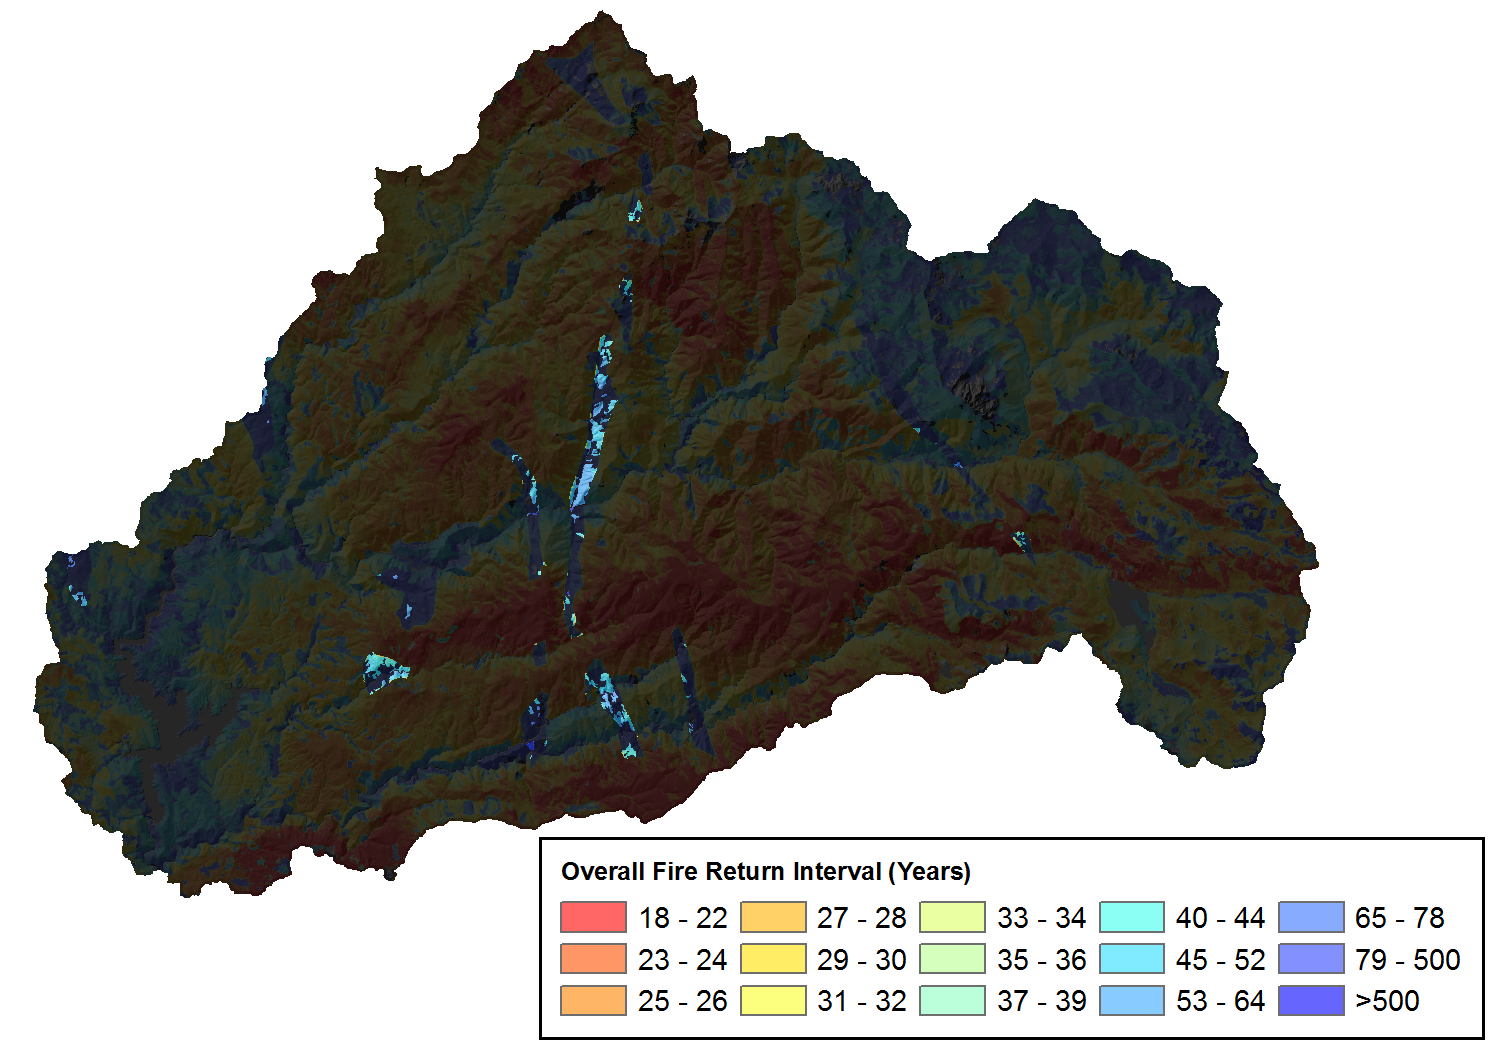
\includegraphics[width=0.5\textwidth]{/Users/mmallek/Tahoe/Report2/images/fri_ocfwu.png}
    }
  \caption{(a) Population return interval (average number of years between fires) distribution for Oak-Conifer Forest and Woodland - Ultramafic.  (b) Spatial depiction of fire return intervals across the landscape. Cover types other than Oak-Conifer Forest and Woodland - Ultramafic are partially obscured in grey. The value at any given cell is the point-specific return interval, which ranges from 21 years to \textgreater 1000 years.}
\label{fig:preturn_ocfwu}
\end{figure}

\begin{figure}[!htbp]
  \centering
  \subfloat[][]{
    \centering
    \includegraphics[width=0.5\textwidth]{/Users/mmallek/Tahoe/R/Rplots/November2014/preturn_rfrm.png}
    }%
  \subfloat[][]{
    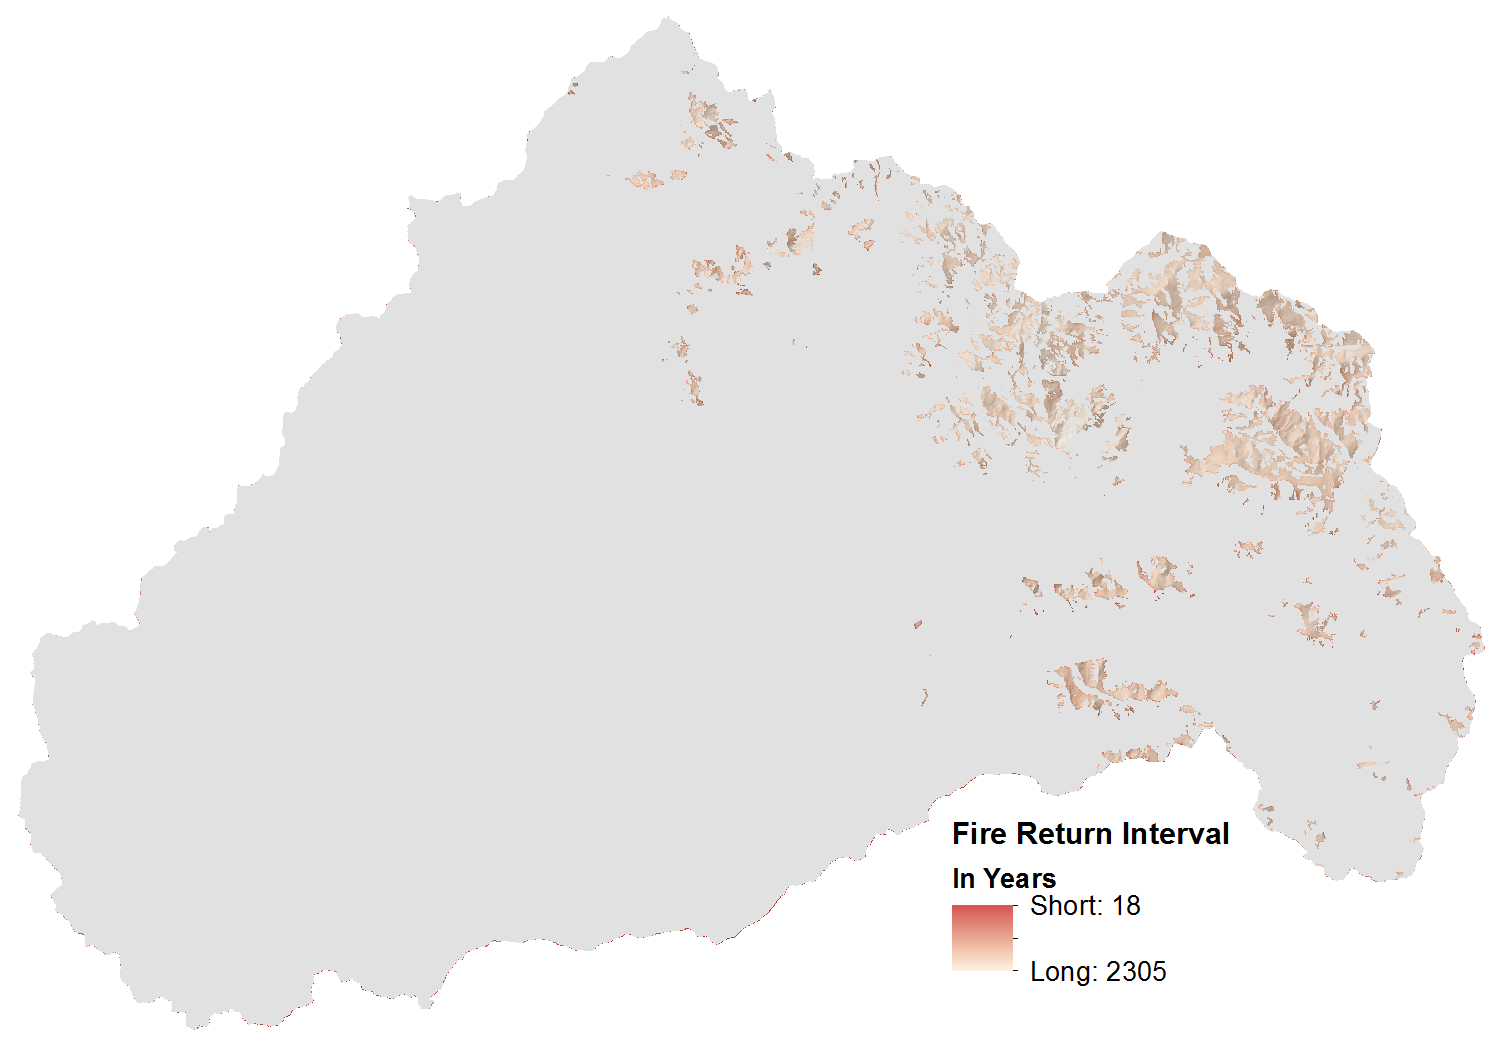
\includegraphics[width=0.5\textwidth]{/Users/mmallek/Tahoe/Report2/images/fri_rfrm.png}
    }
  \caption{(a) Population return interval (average number of years between fires) distribution for Red Fir - Mesic.  (b) Spatial depiction of fire return intervals across the landscape. Cover types other than Red Fir - Mesic are partially obscured in grey. The value at any given cell is the point-specific return interval, which ranges from 21 years to \textgreater 1000 years.}
\label{fig:preturn_rfrm}
\end{figure}

\begin{figure}[!htbp]
  \centering
  \subfloat[][]{
    \centering
    \includegraphics[width=0.5\textwidth]{/Users/mmallek/Tahoe/R/Rplots/November2014/preturn_rfrx.png}
    }%
  \subfloat[][]{
    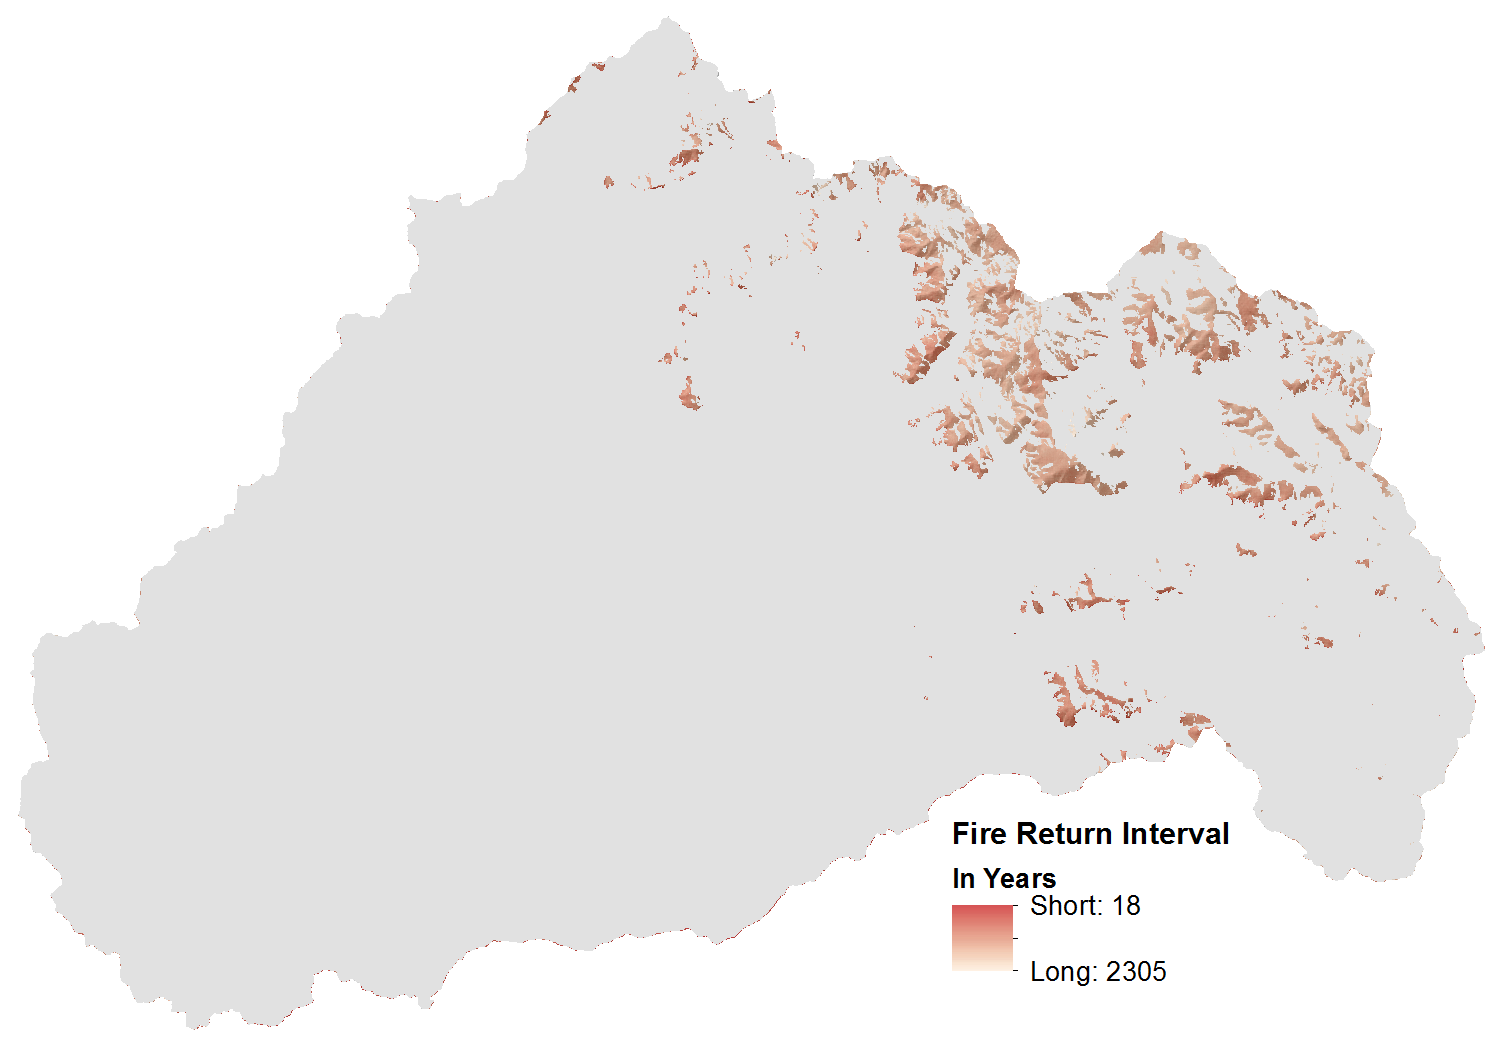
\includegraphics[width=0.5\textwidth]{/Users/mmallek/Tahoe/Report2/images/fri_rfrx.png}
    }
  \caption{(a) Population return interval (average number of years between fires) distribution for Red Fir - Xeric.  (b) Spatial depiction of fire return intervals across the landscape. Cover types other than Red Fir - Xeric are partially obscured in grey. The value at any given cell is the point-specific return interval, which ranges from 20 years to \textgreater 1000 years.}
\label{fig:preturn_rfrx}
\end{figure}

\begin{figure}[!htbp]
  \centering
  \subfloat[][]{
    \centering
    \includegraphics[width=0.5\textwidth]{/Users/mmallek/Tahoe/R/Rplots/November2014/preturn_smcm.png}
    }%
  \subfloat[][]{
    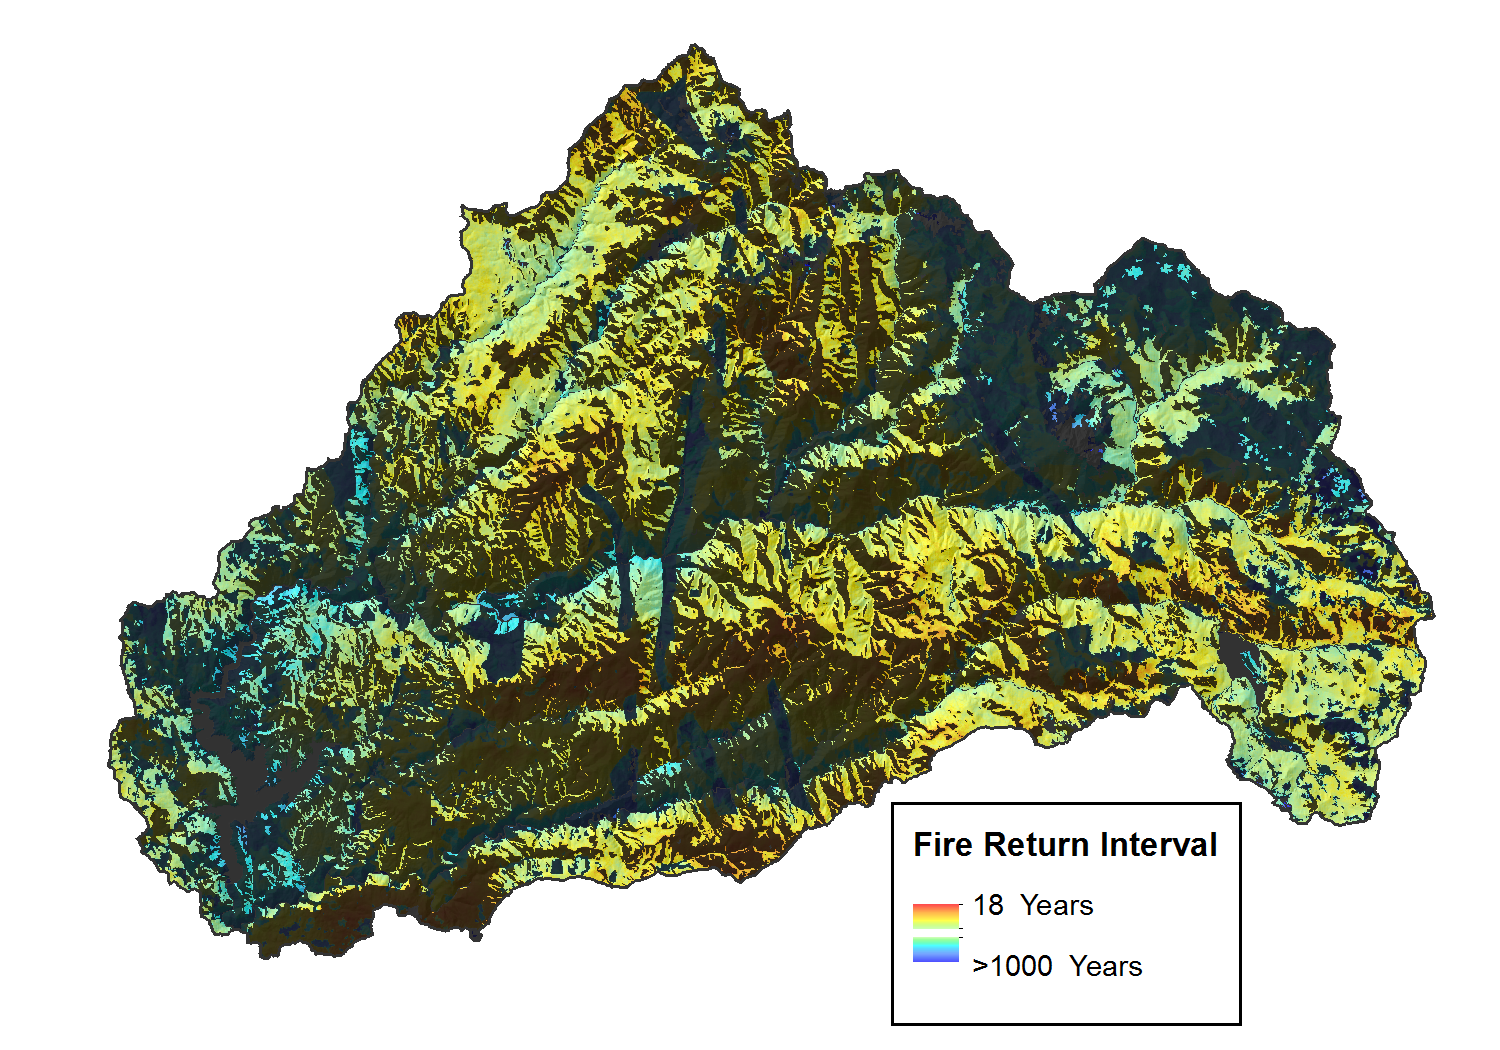
\includegraphics[width=0.5\textwidth]{/Users/mmallek/Tahoe/Report2/images/fri_smcm.png}
    }
  \caption{(a) Population return interval (average number of years between fires) distribution for Sierran Mixed Conifer - Mesic.  (b) Spatial depiction of fire return intervals across the landscape. Cover types other than Sierran Mixed Conifer - Mesic are partially obscured in grey. The value at any given cell is the point-specific return interval, which ranges from 18 years to \textgreater 1000 years.}
\label{fig:preturn_smcm}
\end{figure}

\begin{figure}[!htbp]
  \centering
  \subfloat[][]{
    \centering
    \includegraphics[width=0.5\textwidth]{/Users/mmallek/Tahoe/R/Rplots/November2014/preturn_smcu.png}
    }%
  \subfloat[][]{
    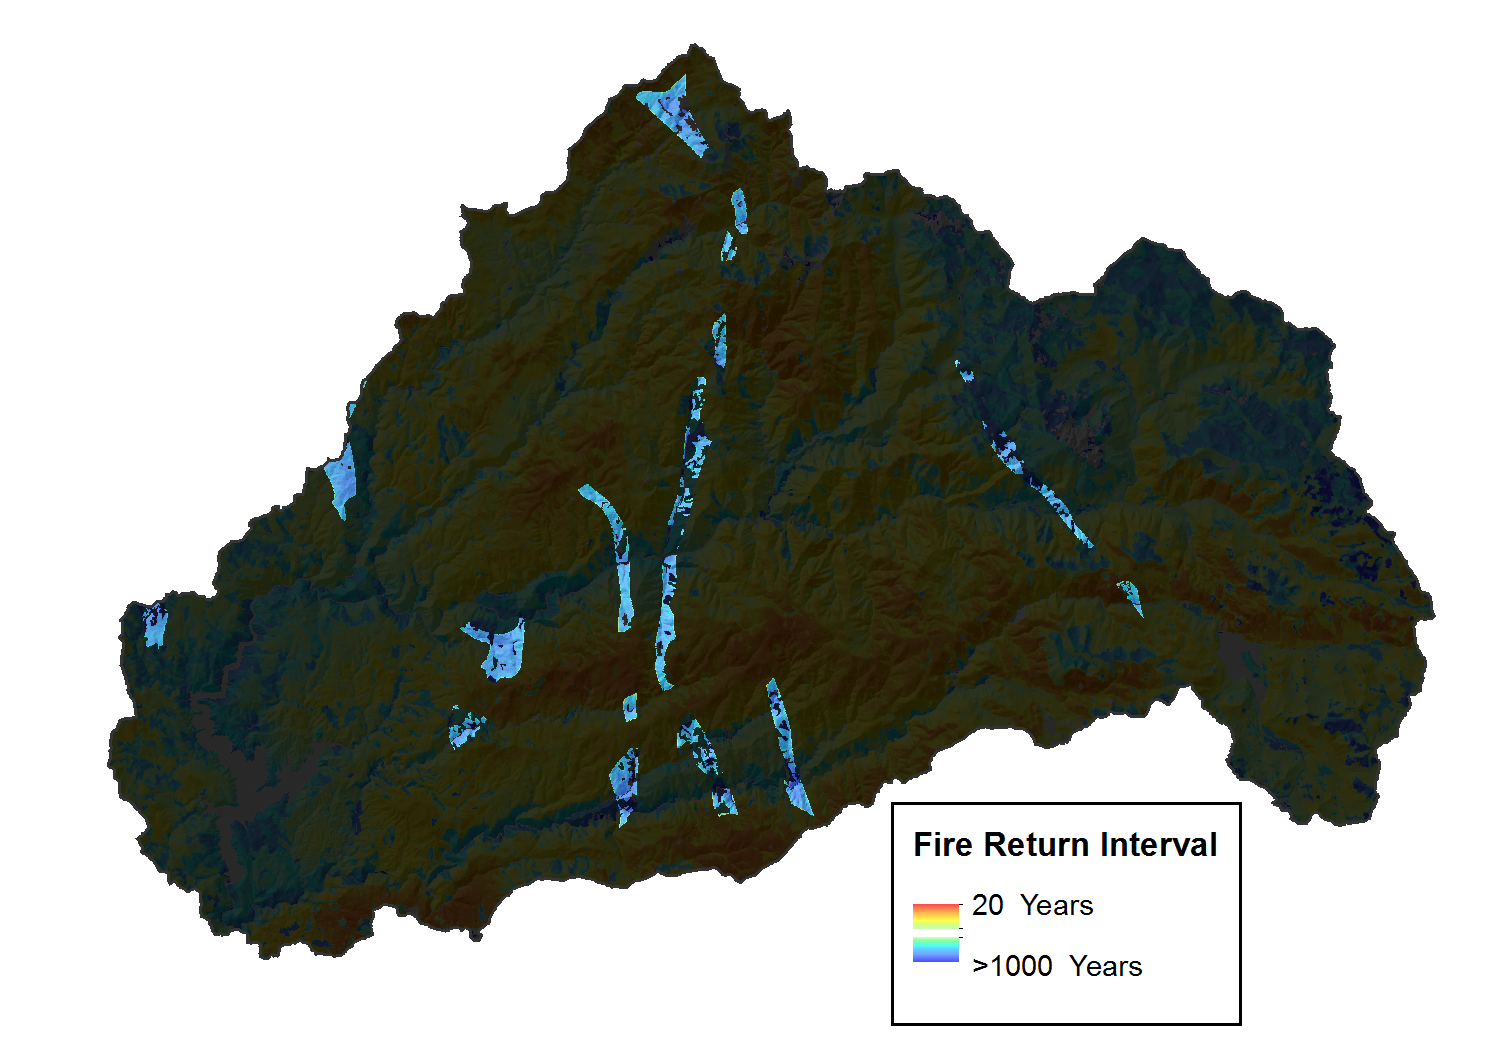
\includegraphics[width=0.5\textwidth]{/Users/mmallek/Tahoe/Report2/images/fri_smcu.png}
    }
  \caption{(a) Population return interval (average number of years between fires) distribution for Sierran Mixed Conifer - Ultramafic.  (b) Spatial depiction of fire return intervals across the landscape. Cover types other than Sierran Mixed Conifer - Ultramafic are partially obscured in grey. The value at any given cell is the point-specific return interval, which ranges from 20 years to \textgreater 1000 years.}
\label{fig:preturn_smcu}
\end{figure}

\begin{figure}[!htbp]
  \centering
  \subfloat[][]{
    \centering
    \includegraphics[width=0.5\textwidth]{/Users/mmallek/Tahoe/R/Rplots/November2014/preturn_smcx.png}
    }%
  \subfloat[][]{
    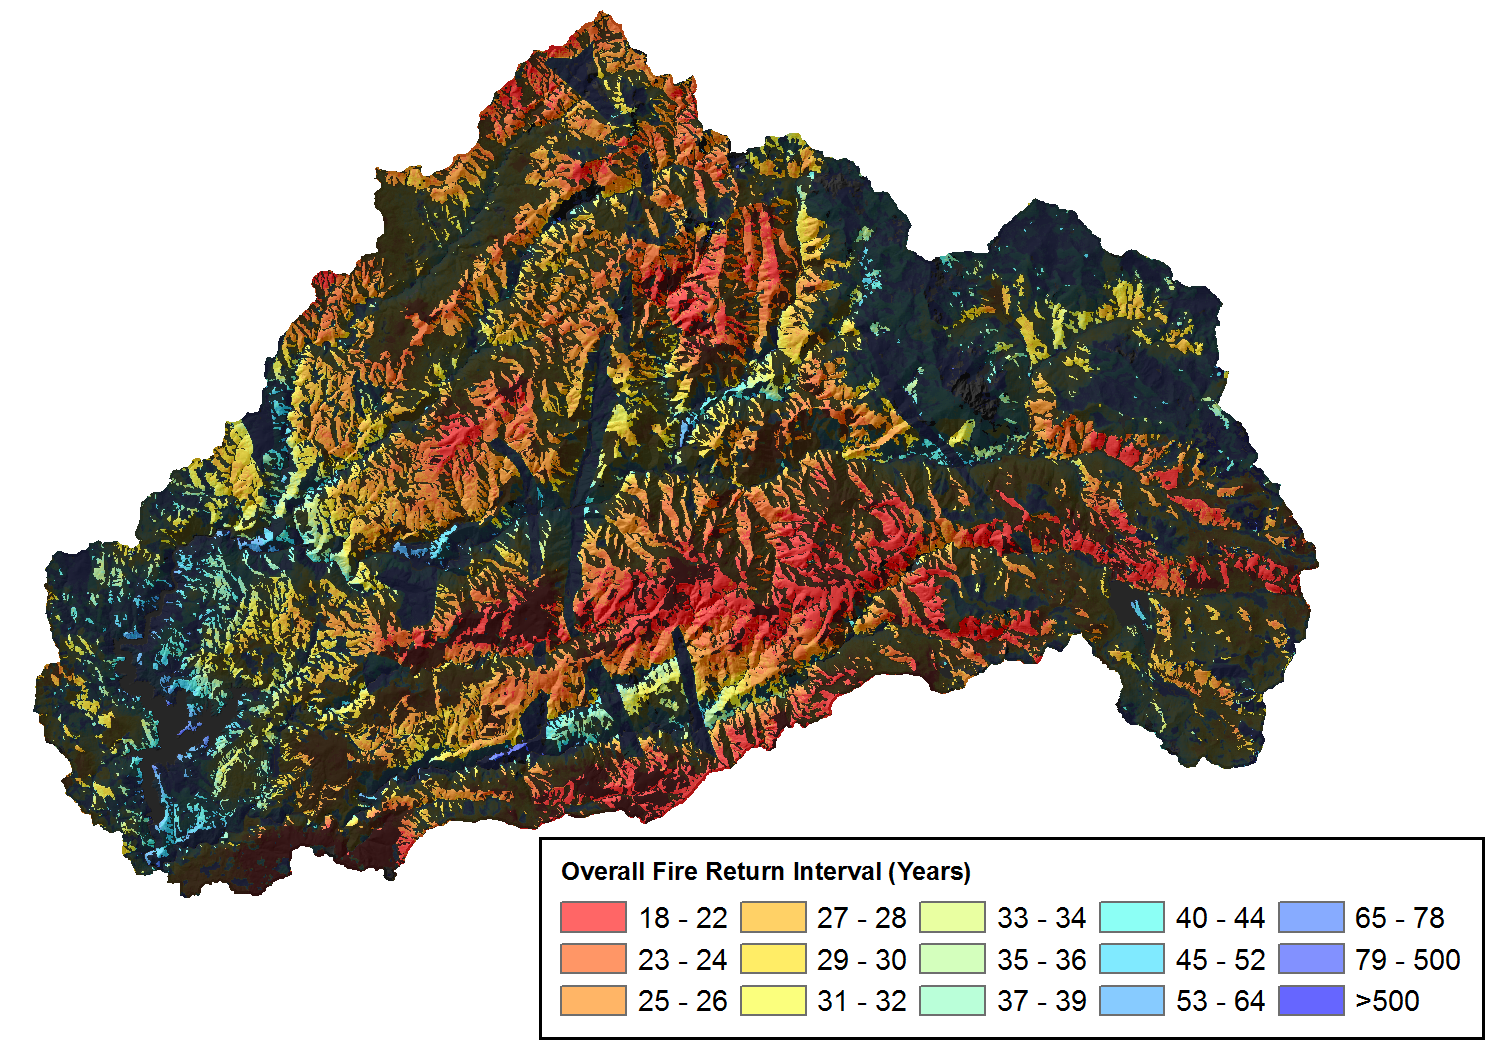
\includegraphics[width=0.5\textwidth]{/Users/mmallek/Tahoe/Report2/images/fri_smcx.png}
    }
  \caption{(a) Population return interval (average number of years between fires) distribution for Sierran Mixed Conifer - Xeric.  (b) Spatial depiction of fire return intervals across the landscape. Cover types other than Sierran Mixed Conifer - Xeric are partially obscured in grey. The value at any given cell is the point-specific return interval, which ranges from 18 years to \textgreater 1000 years.}
\label{fig:preturn_smcx}
\end{figure}

%%%%%%%%%%%%%%%%%%%%%%%%%%%%%%%%
%%%%%%%%%%%%%%%%%%%%%%%%%%%%%%%%
%%%%%%%%%%%%%%%%%%%%%%%%%%%%%%%%
\newpage
\subsection{Vegetation Response}
\label{subsec:HRVvegresponse}

\paragraph{Landscape Composition}

The distribution of area among condition classes within all cover types fluctuated over time, as expected. The relative proportion of each condition class also varied across cover types. In general, the condition class distribution appeared to be in dynamic equilibrium, despite considerable variability from timestep to timestep. 

\begin{figure}[!htbp]
  \centering
  \subfloat[][]{
    \centering
    \includegraphics[width=0.6\textwidth]{/Users/mmallek/Tahoe/R/Rplots/November2014/covcond_megm.png}
    }%
  \subfloat[][]{
  \centering
  \includegraphics[height=2.5in]{/Users/mmallek/Tahoe/R/Rplots/November2014/covcond_current_megm.png}
    }
  \caption{(a) Cover-Condition dynamics for Mixed Evergreen - Mesic. The black vertical line at 40 timesteps marks the end of the equilibration period used in this study. (b) Current seral stage distribution for Mixed Evergreen - Mesic.}
\label{fig:covcond_megm}
\end{figure}

\begin{figure}[!htbp]
  \centering
  \subfloat[][]{
    \centering
    \includegraphics[width=0.6\textwidth]{/Users/mmallek/Tahoe/R/Rplots/November2014/covcond_megx.png}
    }%
  \subfloat[][]{
    \includegraphics[height=2.5in]{/Users/mmallek/Tahoe/R/Rplots/November2014/covcond_current_megx.png}
    }
  \caption{(a) Cover-Condition dynamics for Mixed Evergreen - Xeric. The black vertical line at 40 timesteps marks the end of the equilibration period used in this study. (b) Current seral stage distribution for Mixed Evergreen - Xeric.} 
  \label{fig:covcond_megx}
\end{figure}

\begin{figure}[!htbp]
  \centering
  \subfloat[][]{
    \centering
    \includegraphics[width=0.6\textwidth]{/Users/mmallek/Tahoe/R/Rplots/November2014/covcond_ocfw.png}
    }%
  \subfloat[][]{
    \includegraphics[height=2.5in]{/Users/mmallek/Tahoe/R/Rplots/November2014/covcond_current_ocfw.png}
    }
  \caption{(a) Cover-Condition dynamics for Oak-Conifer Forest and Woodland. The black vertical line at 40 timesteps marks the end of the equilibration period used in this study. (b) Current seral stage distribution for Oak-Conifer Forest and Woodland.} 
  \label{fig:covcond_ocfw}
\end{figure}

\begin{figure}[!htbp]
  \centering
  \subfloat[][]{
    \centering
    \includegraphics[width=0.6\textwidth]{/Users/mmallek/Tahoe/R/Rplots/November2014/covcond_ocfwu.png}
    }%
  \subfloat[][]{
    \includegraphics[height=2.5in]{/Users/mmallek/Tahoe/R/Rplots/November2014/covcond_current_ocfwu.png}
    }
  \caption{(a) Cover-Condition dynamics for Oak-Conifer Forest and Woodland - Ultramafic. The black vertical line at 40 timesteps marks the end of the equilibration period used in this study. (b) Current seral stage distribution for Oak-Conifer Forest and Woodland - Ultramafic.} 
  \label{fig:covcond_ocfwu}
\end{figure}

\begin{figure}[!htbp]
  \centering
  \subfloat[][]{
    \centering
    \includegraphics[width=0.6\textwidth]{/Users/mmallek/Tahoe/R/Rplots/November2014/covcond_rfrm.png}
    }%
  \subfloat[][]{
    \includegraphics[height=2.5in]{/Users/mmallek/Tahoe/R/Rplots/November2014/covcond_current_rfrm.png}
    }
  \caption{(a) Cover-Condition dynamics for Red Fir - Mesic. The black vertical line at 40 timesteps marks the end of the equilibration period used in this study. (b) Current seral stage distribution for Red Fir - Mesic.} 
  \label{fig:covcond_rfrm}
\end{figure}

\begin{figure}[!htbp]
  \centering
  \subfloat[][]{
    \centering
    \includegraphics[width=0.6\textwidth]{/Users/mmallek/Tahoe/R/Rplots/November2014/covcond_rfrx.png}
    }%
  \subfloat[][]{
    \includegraphics[height=2.5in]{/Users/mmallek/Tahoe/R/Rplots/November2014/covcond_current_rfrx.png}
    }
  \caption{(a) Cover-Condition dynamics for Red Fir - Xeric. The black vertical line at 40 timesteps marks the end of the equilibration period used in this study. (b) Current seral stage distribution for Red Fir - Xeric.} 
  \label{fig:covcond_rfrx}
\end{figure}

\begin{figure}[!htbp]
  \centering
  \subfloat[][]{
    \centering
    \includegraphics[width=0.6\textwidth]{/Users/mmallek/Tahoe/R/Rplots/November2014/covcond_smcm.png}
    }%
  \subfloat[][]{
    \includegraphics[height=2.5in]{/Users/mmallek/Tahoe/R/Rplots/November2014/covcond_current_smcm.png}
    }
  \caption{(a) Cover-Condition dynamics for Sierran Mixed Conifer - Mesic. The black vertical line at 40 timesteps marks the end of the equilibration period used in this study. (b) Current seral stage distribution for Sierran Mixed Conifer - Mesic.} 
  \label{fig:covcond_smcm}
\end{figure}

\begin{figure}[!htbp]
  \centering
  \subfloat[][]{
    \centering
    \includegraphics[width=0.6\textwidth]{/Users/mmallek/Tahoe/R/Rplots/November2014/covcond_smcu.png}
    }%
  \subfloat[][]{
    \includegraphics[height=2.5in]{/Users/mmallek/Tahoe/R/Rplots/November2014/covcond_current_smcu.png}
    }
  \caption{(a) Cover-Condition dynamics for Sierran Mixed Conifer - Ultramafic. The black vertical line at 40 timesteps marks the end of the equilibration period used in this study. (b) Current seral stage distribution for Sierran Mixed Conifer - Ultramafic.} 
  \label{fig:covcond_smcu}
\end{figure}

\begin{figure}[!htbp]
  \centering
  \subfloat[][]{
    \centering
    \includegraphics[width=0.6\textwidth]{/Users/mmallek/Tahoe/R/Rplots/November2014/covcond_smcx.png}
    }%
  \subfloat[][]{
    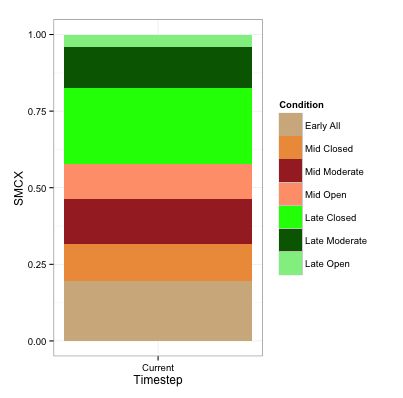
\includegraphics[height=2.5in]{/Users/mmallek/Tahoe/R/Rplots/November2014/covcond_current_smcx.png}
    }
  \caption{(a) Cover-Condition dynamics for Sierran Mixed Conifer - Xeric. The black vertical line at 40 timesteps marks the end of the equilibration period used in this study. (b) Current seral stage distribution for Sierran Mixed Conifer - Xeric.} 
  \label{fig:covcond_smcx}
\end{figure}

%\clearpage

\paragraph{Landscape Structure and Patterns}

The departure index indicates the distance from the 50th percentile value for a given metric. Thus, for the landscape metric 'PD,' 19.507 is equivalent to the 28th percentile of observations during the HRV simulation ($50-22 = 28$). This value is within the HRV for the landscape. However, the landscape metric `ED' is 100, because $128.875 > 123.872$, the largest value observed during the HRV simulation. Edge density at the landscape level is outside the HRV.


\textbf{need to add in TECI}
\begin{verbatim}
$`landscape SRV`
   landscape.metric    srv5%   srv50%   srv95%  current.value current.%SRV departure.index
2                ED  116.425  119.488  122.519        128.875          100             100
4           AREA_AM  169.503  194.062  243.753        119.985            0            -100
5         GYRATE_AM  714.212  752.733  806.692        620.951            0            -100
7          SHAPE_AM    3.604    3.776    3.988          3.243            0            -100
9           CORE_AM  146.748  167.446  211.455        106.710            0            -100
11          SIMI_MN 2433.125 2683.733 3029.040       2095.764            0            -100
12             CWED   40.169   41.449   42.453         36.092            0            -100
13           CONTAG   54.481   55.222   55.973         51.172            0            -100
16             SIDI    0.936    0.942    0.948          0.962          100             100
17             SIEI    0.944    0.950    0.956          0.971          100             100
18               AI   81.871   82.324   82.791         80.963            0            -100

$`landscape departure index (%)`
[1] 87
\end{verbatim}

Several of the individual landscape metrics are redundant with one another. For example, \emph{Contagion} and \emph{Edge Density} are inversely related, so it is perhaps helpful, but not necessary, to examine both metrics. Here we highlight a subset of the metrics from Table MAKE TABLE for the purposes of discussing the landscape under the simulated historic period as compared to the present day.

First, we note that during the HRV, the landscape was composed of larger and more extensive patches, as illustrated by Figure \ref{landscapestory1}. 
Second, patches on the landscape were more aggregated at the cell-level during HRV, which is illustrated by the \emph{Contagion} metric. In addition, we observe increased dominance by certain cover types, as illustrated by smaller values for the \emph{Simpson's Evenness Index} durin the HRV (see Figure \ref{landscapestory2}). However, despite being larger, more extensive, and aggregated, they do not show an associated increase in core area. This indicates that they are geometrically more complex, to the extent that little core area fits inside each patch. As an example, we highlight in Figure \ref{landscapestory3} a patch of Sierran Mixed Conifer - Mesic Forest in the Mid Development - Closed condition, which is one of the largest patches on the landscape. Little room is available for cores due to the irregular shape of this patch.


\begin{figure}
\includegraphics[width=0.5\textwidth]{/Users/mmallek/Tahoe/R/Rplots/November2014/AREA_AM1.png}
\includegraphics[width=0.5\textwidth]{/Users/mmallek/Tahoe/R/Rplots/November2014/SHAPE_AM1.png}
\caption{Landscape \textsc{Fragstats} Metrics. Left, Area-weighted Mean Patch Area. Right, Area-weighted Mean Shape. We use the area-weighted metrics to reduce the influence of the many extremely small patches. The average patch size is large, and the average patch shape more complex, than the current landscape.} 
\label{landscapestory1}
\end{figure}

\begin{figure}
\includegraphics[width=0.5\textwidth]{/Users/mmallek/Tahoe/R/Rplots/November2014/CONTAG1.png}
\includegraphics[width=0.5\textwidth]{/Users/mmallek/Tahoe/R/Rplots/November2014/SIEI1.png}
\caption{Landscape \textsc{Fragstats} Metrics. At left is Contagion, a metric describing patch dispersion and interspersion. The landscape during the HRV is much more contagious than the current landscape. At right is Simpson's Evenness Index, which indicates the distance from maximum diversity, or evenness, in the landscape patches. Values for Simpson's Evenness are near 1 during the HRV and in the present landscape, but the HRV values are well below the current conditions.} 
\label{landscapestory2}
\end{figure}

\begin{figure}
\includegraphics[width=0.5\textwidth]{/Users/mmallek/Tahoe/R/Rplots/November2014/CORE_AM1.png}
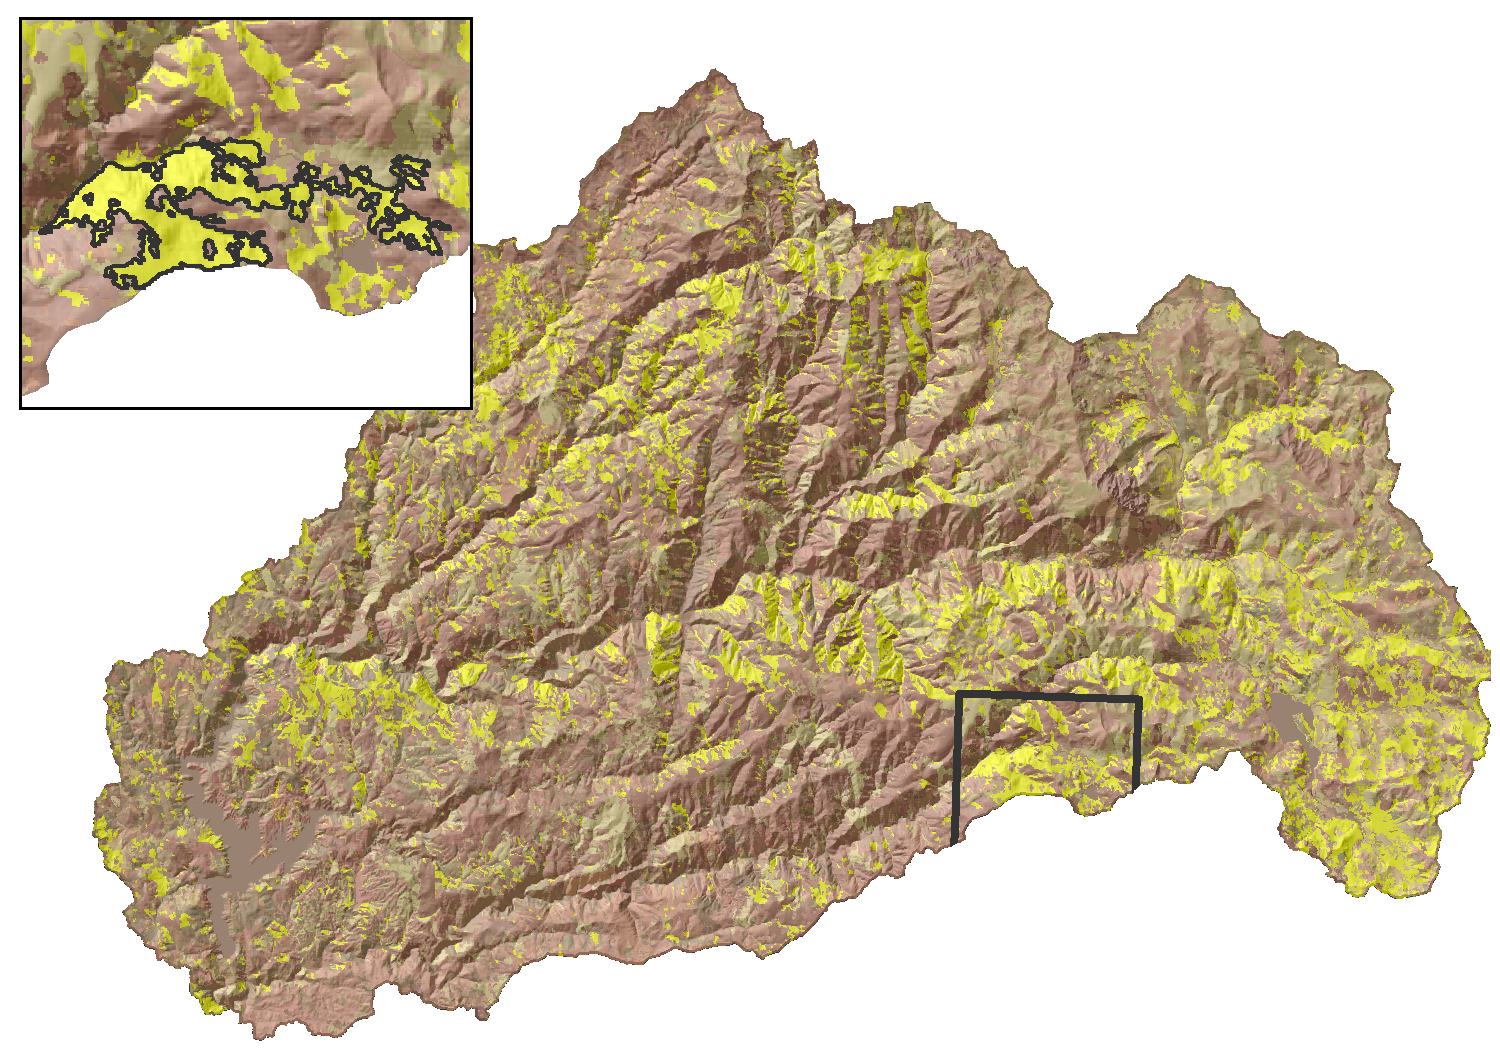
\includegraphics[width=0.5\textwidth]{/Users/mmallek/Tahoe/Report2/images/largepatch_1035_2420}
\caption{Landscape \textsc{Fragstats} Metrics. At left are the results for the Area-weighted Mean Core Area, a measure of interior habitat available at the patch level. At right is an example of a highly complex, albeit very large, patch of Sierran Mixed Conifer - Mesic, Mid Development - Closed, habitat. All patches of this type are highlighted as yellow; other patch types appear in earth tones. The zoomed-in image of a single patch illustrates the shape complexity and edge density of such patches, which are common during the HRV simulation.} 
\label{landscapestory3}
\end{figure}

\subsection{Historic Range of Variability Departure}
\paragraph{Landscape-level Results}
One of the principal purposes of gaining a better quantitative understanding of the historic reference period is to know whether recent human activities have caused landscapes to move outside their historic range of variability (Landres et al.1999; Swetnam et al. 1999). As described above, we summarized the distribution of each metric calculated over the length of the simulation, minus the equilibration period. We computed the $0^{th}$, $5^{th}$, $25^{th}$, $50^{th}$, $75^{th}$, $95^{th}$ and $100^{th}$ percentiles of the distribution of observed values. The current percentile for the statistical range of variability refers to the place within the $0-100^{th}$ percentile of the observed, simulated HRV. If the current value is outside the HRV, it is given the appropriate maximum (100) or minimum (0) score. The index of departure from HRV measures the relative distance from the median HRV value to the $0^{th}$ or $100^{th}$ percentile. At the landscape-level, most computed metrics have values outside the HRV. 

\begin{verbatim}
$`landscape SRV`
landscape.metric    srv0%    srv5%   srv25%   srv50%   srv75%   srv95%  srv100% srv.cv current.value current.%SRV departure.index
              PD   17.866   18.647   19.211   19.679   20.229   20.872   21.372     11        19.507           39             -22
              ED  114.606  116.425  118.376  119.488  120.683  122.519  123.872      5       128.875          100             100
         AREA_MN    4.679    4.791    4.943    5.082    5.205    5.363    5.597     11         5.126           61              22
         AREA_AM  158.590  169.503  183.793  194.062  209.983  243.753  362.032     38       119.985            0            -100
       GYRATE_AM  693.818  714.212  737.307  752.733  770.930  806.692  914.181     12       620.951            0            -100
        SHAPE_MN    1.411    1.416    1.421    1.426    1.432    1.439    1.444      2         1.511          100             100
        SHAPE_AM    3.547    3.604    3.712    3.776    3.860    3.988    4.272     10         3.243            0            -100
         CORE_MN    2.921    3.018    3.096    3.175    3.251    3.361    3.515     11         3.347           95              90
         CORE_AM  137.672  146.748  157.365  167.446  181.671  211.455  329.638     39       106.710            0            -100
          CAI_AM   59.851   60.638   61.606   62.467   63.422   64.833   66.444      7        65.295           98              96
         SIMI_MN 2316.796 2433.125 2575.450 2683.733 2801.744 3029.040 3918.372     22      2095.764            0            -100
            CWED   39.586   40.169   40.889   41.449   41.936   42.453   43.513      6        36.092            0            -100
          CONTAG   54.205   54.481   54.874   55.222   55.605   55.973   56.647      3        51.172            0            -100
             IJI   60.367   61.568   62.217   62.697   63.199   63.876   64.361      4        65.868          100             100
            SIDI    0.932    0.936    0.939    0.942    0.944    0.948    0.951      1         0.962          100             100
            SIEI    0.940    0.944    0.947    0.950    0.952    0.956    0.959      1         0.971          100             100
              AI   81.664   81.871   82.142   82.324   82.493   82.791   83.061      1        80.963            0            -100

$`landscape departure index (%)`
[1] 87
\end{verbatim}

\paragraph{Class-level Results} We compiled the results for several class-level metrics for a few classes of particular interest. \textbf{I don't fully understand why the class-level results are not as useful to report.} We were particularly interested in the Early Development condition for Sierran Mixed Conifer - Mesic, Sierran Mixed Conifer - Xeric, and Oak-Conifer Forest and Woodland, cover types that are very extensive across our landscape, are predicted to be highly affected by past fire suppression, and are characterized by chaparral vegetation present during the early successional stage. The results differ across the three cover types. Oak-Conifer Forest and Woodland's early seral patches are, on average, smaller, less complex, and less aggregated today than during the HRV, although this is in relation to the median values rather than the HRV. Current values are within HRV for all but one metric, Mean Similarity. For Sierran Mixed Conifer - Mesic, early seral patches are smaller, less complex, and less aggregated than during HRV, but their departure from the median is greater. Four metrics are outside of the $5^{th}-95^{th}$ percentile range, including Area-weighted Mean Area and Area-weighte Mean Core Area. Sierran Mixed Conifer - Xeric patches in the early seral stage show the greatest departure among the three: virtually all metrics are outside the HRV. Each metric is also less than the HRV, indicating that patches today are smaller, simpler and more dispersed and disjunct from one another than during the HRV.

\begin{verbatim}

OCFW_EARLY_ALL                      
class.metric  srv0%   srv5%     srv25%    srv50%    srv75%    srv95%    srv100%   srv.cv  current.value current.%SRV  departure.index
PLAND         0.336   1.075     1.611     2.114     2.655     3.414     4.038     111     2.556         73            46
PD            0.066   0.157     0.226     0.281     0.34      0.423     0.469     95      0.348         78            56
ED            0.788   2.136     3.245     4.071     5.03      6.324     7.179     103     5.472         81            62
AREA_AM       14.188  31.898    53.709    75.523    121.551   257.481   690.206   299     45.113        17            -66
GYRATE_AM     154.862 226.585   286.262   335.971   419.323   619.563   1304.257  117     268.668       19            -62
SHAPE_AM      1.667   1.894     2.081     2.281     2.542     3.202     4.368     57      2.069         22            -56
CPLAND        0.316   1.046     1.551     2.022     2.554     3.277     3.868     110     2.49          75            50
CORE_AM       13.693  30.715    51.446    71.899    115.099   248.712   622.361   303     43.871        17            -66
SIMI_MN       2263.72 2944.843  3396.432  3717.607  4129.621  4821.523  5971.134  50      2409.316      1             -98
CWED          0.3     0.842     1.218     1.524     1.863     2.333     2.692     98      1.905         76            52
CLUMPY        0.81    0.83      0.845     0.853     0.863     0.875     0.888     5       0.837         12            -76
IJI           57.218  59.396    61.201    62.526    63.826    65.382    67.954    10      60.61         17            -66
AI            81.221  83.224    84.799    85.643    86.611    87.819    88.984    5       84.16         14            -72
                      
SMC_M_EARLY_ALL                     
class.metric  srv0% srv5% srv25%  srv50%  srv75%  srv95%  srv100% srv.cv  current.value current.%SRV  departure.index
PLAND 1.169 2.423 3.824 5.144 6.687 8.713 11.135  122 4.734 42  -16
PD  0.29  0.566 0.828 1.018 1.285 1.651 1.83  107 1.079 56  12
ED  3.221 6.039 9.406 12.089  15.556  20.002  22.576  116 12.896  57  14
AREA_AM 12.982  36.582  64.066  107.019 177.143 322.34  492.634 267 28.587  2 -96
GYRATE_AM 144.368 246.699 319.422 393.868 497.731 672.406 883.739 108 235.351 4 -92
SHAPE_AM  1.808 2.254 2.551 2.85  3.204 3.806 4.5 54  2.295 8 -84
CPLAND  1.107 2.308 3.636 4.871 6.335 8.234 10.456  122 4.567 43  -14
CORE_AM 12.703  34.674  61.811  101.666 171.559 306.569 477.974 267 27.758  2 -96
SIMI_MN 2582.235  3209.307  3740.451  4055.179  4370.167  4847.816  5567.094  40  2306.563  0 -100
CWED  0.998 1.934 3.022 3.818 4.83  6.057 7.091 108 3.67  44  -12
CLUMPY  0.758 0.789 0.801 0.812 0.823 0.837 0.852 6 0.786 5 -90
IJI 54.175  56.443  58.314  59.723  61.171  63.027  65.39 11  56.964  9 -82
AI  76.26 79.676  81.085  82.131  83.404  84.529  85.703  6 79.656  5 -90
                      
SMC_X_EARLY_ALL                     
class.metric  srv0% srv5% srv25%  srv50%  srv75%  srv95%  srv100% srv.cv  current.value current.%SRV  departure.index
PLAND 5.199 7.325 9.002 10.251  11.846  14.373  15.814  69  5.639 1 -98
PD  0.819 1.132 1.315 1.462 1.605 1.734 1.839 41  1.029 2 -96
ED  11.207  15.721  18.64 21.113  24.003  27.463  29.289  56  13.431  2 -96
AREA_AM 61.641  84.446  103.061 141.611 199.919 434.898 514.704 247 75.911  2 -96
GYRATE_AM 331.499 384.382 421.969 493.15  585.283 752.269 856.6 75  327.449 0 -100
SHAPE_AM  2.582 2.827 3.03  3.249 3.604 4.273 4.441 45  2.596 1 -98
CPLAND  5.008 7.13  8.711 9.933 11.475  13.946  15.369  69  5.466 1 -98
CORE_AM 60.465  82.626  100.803 138.936 197.128 430.536 508.524 250 75.189  3 -94
SIMI_MN 2380.781  2628.112  2862.546  3066.171  3259.545  3579.682  3865.676  31  1595.569  0 -100
CWED  4.097 5.721 6.674 7.57  8.611 9.99  11.273  56  4.014 0 -100
CLUMPY  0.815 0.822 0.826 0.829 0.832 0.836 0.843 2 0.812 0 -100
IJI 56.87 60.057  62.352  63.427  64.249  65.036  65.989  8 58.922  2 -96
AI  83.201  83.709  84.26 84.65 85  85.777  86.318  2 82.258  0 -100

\end{verbatim}

Also look at closed forest for RFRM, RFRX, SMCM, SMCX.

\begin{verbatim}
RFR_M_LATE_CL                     
class.metric  srv0% srv5% srv25%  srv50%  srv75%  srv95%  srv100% srv.cv  current.value current.%SRV  departure.index
PLAND 0.898 1.417 1.744 2.019 2.297 2.856 3.23  71  0.508 0 -100
PD  0.192 0.234 0.272 0.301 0.328 0.357 0.377 41  0.122 0 -100
ED  2.307 3.214 3.856 4.463 4.922 5.581 6.434 53  1.49  0 -100
AREA_MN 4.133 5.344 6.037 6.639 7.411 8.723 10.239  51  4.173 1 -98
AREA_AM 26.059  37.406  60.014  85.09 116.663 189.04  332.006 178 13.681  0 -100
GYRATE_AM 214.079 260.799 328.984 409.488 474.527 596.16  746.608 82  167.222 0 -100
SHAPE_MN  1.424 1.45  1.48  1.499 1.515 1.538 1.559 6 1.527 91  82
SHAPE_AM  2.169 2.341 2.727 3.01  3.329 3.81  4.415 49  2.042 0 -100
CPLAND  0.1 0.246 0.423 0.552 0.717 0.93  1.249 124 0.112 1 -98
CORE_MN 0.518 0.949 1.478 1.835 2.32  2.982 3.585 111 0.922 5 -90
CORE_AM 5.131 10.372  21.661  34.43 51.383  100.61  155.982 262 3.666 0 -100
CAI_AM  10.752  16.835  23.55 27.267  31.7  36.348  43.223  72  22.106  19  -62
SIMI_MN 621.767 734.173 853.166 941.771 1070.579  1249.121  1714.258  55  412.672 0 -100
CWED  1.039 1.328 1.555 1.696 1.881 2.173 2.562 50  0.397 0 -100
CLUMPY  0.798 0.819 0.826 0.836 0.843 0.852 0.862 4 0.786 0 -100
IJI 55.409  58.183  60.054  61.56 62.602  64.172  65.944  10  57.207  2 -96
AI  80.031  82.223  82.966  83.928  84.666  85.671  86.537  4 78.708  0 -100

RFR_X_LATE_CL                     
class.metric  srv0% srv5% srv25%  srv50%  srv75%  srv95%  srv100% srv.cv  current.value current.%SRV  departure.index
PLAND 0.131 0.199 0.352 0.528 0.698 1.091 1.493 169 0.43  38  -24
PD  0.09  0.119 0.15  0.183 0.214 0.256 0.287 75  0.101 1 -98
ED  0.511 0.71  1.099 1.529 1.917 2.717 3.467 131 1.221 34  -32
AREA_MN 1.282 1.575 2.316 2.811 3.404 4.467 5.696 103 4.238 92  84
AREA_AM 4.014 6.899 11.395  19.161  30.207  60.391  95.736  279 10.145  16  -68
GYRATE_AM 85.566  109.069 142.201 178.369 217.187 313.02  385.142 114 140.872 24  -52
SHAPE_MN  1.202 1.232 1.284 1.315 1.347 1.396 1.433 12  1.5 100 100
SHAPE_AM  1.476 1.62  1.8 1.988 2.197 2.761 3.115 57  1.839 30  -40
CPLAND  0.006 0.021 0.056 0.103 0.17  0.362 0.636 331 0.128 59  18
CORE_MN 0.061 0.169 0.37  0.569 0.826 1.457 2.224 226 1.259 93  86
CORE_AM 0.238 1.027 2.965 5.909 11.09 24.974  53.279  405 3.631 33  -34
CAI_AM  4.72  9.569 15.292  19.875  25.511  33.917  42.599  123 29.709  88  76
SIMI_MN 599.829 691.174 809.823 920.938 1084.89 1445.601  1701.381  82  421.915 0 -100
CWED  0.204 0.26  0.388 0.498 0.615 0.843 0.987 117 0.281 7 -86
CLUMPY  0.708 0.737 0.769 0.784 0.8 0.819 0.839 10  0.793 65  30
IJI 48.808  50.57 52.067  53.182  54.231  56.373  58.019  11  55.276  88  76
AI  70.826  73.691  77.034  78.543  80.128  82.122  84.087  11  79.354  62  24

SMC_M_LATE_CL                     
class.metric  srv0% srv5% srv25%  srv50%  srv75%  srv95%  srv100% srv.cv  current.value current.%SRV  departure.index
PLAND 0.208 0.961 2.499 3.857 5.177 7.357 9.157 166 7.462 96  92
PD  0.147 0.326 0.659 0.868 1.063 1.363 1.545 119 1.112 79  58
ED  0.841 3.076 6.924 9.93  12.897  17.174  20.386  142 17.012  95  90
AREA_MN 1.353 2.406 3.731 4.321 5.17  6.406 8.423 93  6.71  97  94
AREA_AM 4.789 14.879  54.632  89.688  154.573 315.367 534.571 335 64.791  33  -34
GYRATE_AM 93.644  167.812 300.16  376.588 484.645 709.582 990.619 144 375.073 50  0
SHAPE_MN  1.238 1.36  1.414 1.443 1.465 1.492 1.544 9 1.549 100 100
SHAPE_AM  1.652 2.086 2.677 3.044 3.519 4.495 5.832 79  2.84  37  -26
CPLAND  0.041 0.167 0.693 1.225 1.833 2.864 3.714 220 3.217 99  98
CORE_MN 0.186 0.327 0.99  1.402 1.868 2.668 3.648 167 2.893 98  96
CORE_AM 0.785 3.505 26.799  47.316  87.193  189.815 331.681 394 35.675  36  -28
CAI_AM  7.901 14.485  26.406  32.133  36.718  42.011  49.619  86  43.109  97  94
SIMI_MN 1444.936  1656.418  1858.999  2004.923  2244.838  2655.042  4204.844  50  1675.049  7 -86
CWED  0.319 1.007 2.043 2.928 3.756 4.952 5.923 135 4.36  87  74
CLUMPY  0.704 0.738 0.783 0.798 0.811 0.832 0.848 12  0.817 85  70
IJI 53.615  56.531  58.326  59.844  61.099  63.175  66.345  11  55.973  4 -92
AI  70.502  74.288  78.981  80.614  82.035  83.944  85.525  12  83.088  90  80

SMC_X_LATE_CL                     
class.metric  srv0% srv5% srv25%  srv50%  srv75%  srv95%  srv100% srv.cv  current.value current.%SRV  departure.index
PLAND 0.05  0.235 0.526 1.012 1.651 2.864 3.784 260 7.101 100 100
PD  0.063 0.128 0.253 0.377 0.501 0.779 0.932 173 1.074 100 100
ED  0.222 0.842 1.748 3.098 4.645 7.822 9.774 225 16.329  100 100
AREA_MN 0.797 1.349 2.095 2.798 3.391 4.209 4.884 102 6.612 100 100
AREA_AM 2.916 6.991 15.675  25.018  36.818  65.141  309.824 232 54.859  93  86
GYRATE_AM 71.194  109.255 161.276 204.085 247.911 334.42  622.81  110 337.094 96  92
SHAPE_MN  1.125 1.225 1.284 1.326 1.363 1.394 1.421 13  1.533 100 100
SHAPE_AM  1.42  1.66  1.945 2.148 2.33  2.811 4.073 54  2.679 94  88
CPLAND  0.012 0.051 0.167 0.335 0.64  1.125 1.687 321 3.083 100 100
CORE_MN 0.139 0.284 0.617 0.978 1.305 1.797 2.208 155 2.871 100 100
CORE_AM 0.888 2.585 6.93  12.611  19.754  36.415  197.994 268 28.765  91  82
CAI_AM  12.183  20.266  29.303  34.889  39.107  44.925  50.113  71  43.422  93  86
SIMI_MN 1189.343  1394.257  1627.227  1840.696  2066.353  2580.536  5531.82 64  1315.297  3 -94
CWED  0.081 0.241 0.454 0.768 1.134 1.949 2.441 222 3.952 100 100
CLUMPY  0.663 0.712 0.754 0.781 0.795 0.809 0.833 12  0.816 99  98
IJI 50.169  52.818  55.013  56.392  58.036  59.9  63.038  13  54.806  23  -54
AI  66.362  71.254  75.6  78.324  79.874  81.382  83.481  13  82.938  100 100
\end{verbatim}

\section{Future Vegetation Management Scenarios}

%%%%%%%%%%%%%%%%%%%%%%%%%%%%%%%%%%%%%%
%%% original writeup of metric results
%%%%%%%%%%%%%%%%%%%%%%%%%%%%%%%%%%%%%%
%
%\begin{figure}
%\includegraphics[width=0.5\textwidth]{/Users/mmallek/Tahoe/R/Rplots/November2014/ED1.png}
%\includegraphics[width=0.5\textwidth]{/Users/mmallek/Tahoe/R/Rplots/November2014/PD1.png}
%\caption{Landscape structure dynamics} 
%%\label{covcond_smcx}
%\end{figure}
%
%Edge density now is much lower than the HRV. This means the current landscape has more edge. This may be due to the presence of smaller fires overall %recently, and to timber management, both of which could contribute to increased edge. 
%
%Patch density is about the same. Since this is a landscape metric, the means only that the number of patches is within the HRV. The fact that this in %in HRV and ED is outside HRV indicates that patch sizes have gotten less complicated. This metric may also be confounded by the minimum-maximum %possible patches based on the cover types alone (?).
%
%\begin{figure}
%\includegraphics[width=0.5\textwidth]{/Users/mmallek/Tahoe/R/Rplots/November2014/AREA_MN1.png}
%\includegraphics[height=2.5in]{/Users/mmallek/Tahoe/R/Rplots/November2014/AREA_AM1.png}
%\caption{Landscape structure dynamics} 
%%\label{covcond_smcx}
%\end{figure}
%
%AREA\_MN don't think we want. Result makes sense given similar patch numbers. But the AREA\_AM gets at something important, which is that the %distribution of patch sizes is not the same. Proportionally, there are more larger patches during HRV than in the current snapshot. Once during the %simulation some really large patches were generated, but for the most part the graph seems stable around a $100m^2$ mean patch size on the landscape.
%
%\begin{figure}
%\includegraphics[width=0.5\textwidth]{/Users/mmallek/Tahoe/R/Rplots/November2014/GYRATE_AM1.png}
%\includegraphics[height=2.5in]{/Users/mmallek/Tahoe/R/Rplots/November2014/CAI_AM1.png}
%\caption{Landscape structure dynamics} 
%%\label{covcond_smcx}
%\end{figure}
%
%Area-weighted gyration is telling us about the same thing as the area-weight patch size. Not sure if there is a way to compare the length to the %length that would exist if all the patches were square.
%
%The area-weighted core area index indicates that core areas during the HRV were generally smaller than they are now. Again would be nice to have %bounds on the min and max core area based on configuration of cover types. The might not be that useful a metric at the landscape scale.  
%
%\begin{figure}
%\includegraphics[width=0.5\textwidth]{/Users/mmallek/Tahoe/R/Rplots/November2014/CORE_MN1.png}
%\includegraphics[height=2.5in]{/Users/mmallek/Tahoe/R/Rplots/November2014/CORE_AM1.png}
%\caption{Landscape structure dynamics} 
%%\label{covcond_smcx}
%\end{figure}
%
%Core is the area in cores. Current landscape is at about the 94th percentile of HRV. Generally, the average core size was a bit lower during the %historic period. But, if we add area-based weighting, then the core area was a lot higher during HRV. One reason for this could be that there are a %lot of smaller patches, with correspondingly small cores, that tend to get disturbed or react to disturbance uniformly, for probably a variety of %reasons. These patches could contribute to similarities between HRV and current conditions. However, the larger patches on the landscape, when given %more weight, show that conditions currently are pretty different from the simulated HRV. This area-weighted mean core area doesn't tell us anything %too different from the area-weighted mean patch size, though.
%
%\begin{figure}
%\includegraphics[width=0.5\textwidth]{/Users/mmallek/Tahoe/R/Rplots/November2014/SHAPE_MN1.png}
%\includegraphics[height=2.5in]{/Users/mmallek/Tahoe/R/Rplots/November2014/SHAPE_AM1.png}
%\caption{Landscape structure dynamics} 
%%\label{covcond_smcx}
%\end{figure}
%
%Average shape complexity is higher in the current landscape. We saw this same phenomenon in the edge density. But the area-weighted mean value is also %very different from the simulated data. In that case, the shape complexity is higher in the simulated landscapes. This probably means that the largest %patches in the simulated landscape were more complex shape-wise. I'm not sure what metric would tell us the range of values for area - might have to %rerun fragstats to get that.
%
%\begin{figure}
%\includegraphics[width=0.5\textwidth]{/Users/mmallek/Tahoe/R/Rplots/November2014/SIMI_MN1.png}
%\includegraphics[height=2.5in]{/Users/mmallek/Tahoe/R/Rplots/November2014/CWED1.png}
%\caption{Landscape structure dynamics} 
%%\label{covcond_smcx}
%\end{figure}
%
%Results for the similarity index indicate that patches in the simulated landscape tend to be similar to their neighbors compared to the current %landscape. The simulated landscape has more larger, similar patches. This correlates with the other set of results that cover type is often a %predictor of condition class.
%
%Contrast-weighted Edge Density is much higher for the HRV than current, which differs from the ED results. This indicates that the contrast between %patch types is higher in the HRV simulation. Current CWED is quite low.
%
%\begin{figure}
%\includegraphics[width=0.5\textwidth]{/Users/mmallek/Tahoe/R/Rplots/November2014/CONTAG1.png}
%\includegraphics[height=2.5in]{/Users/mmallek/Tahoe/R/Rplots/November2014/IJI1.png}
%\caption{Landscape structure dynamics} 
%%\label{covcond_smcx}
%\end{figure}
%
%The likelihood of a cell on the landscape having a cell of the same patch type next to it is much higher for the simulated HRV than for the current %landscape. This fits with the results of the other similarity metrics saying the HRV landscape had more similarity among patch types. 
%
%The IJI should be larger as the landscape has more of a salt and pepper effect. IJI looks at the patch level rather than the cell level. These results %confirm the others: the current landscape is more interspersed - more salt and pepper-like - than the HRV landscape, which is more aggregated and %clumpy.
%
%\begin{figure}
%\includegraphics[width=0.5\textwidth]{/Users/mmallek/Tahoe/R/Rplots/November2014/SIDI1.png}
%\includegraphics[height=2.5in]{/Users/mmallek/Tahoe/R/Rplots/November2014/SIEI1.png}
%\caption{Landscape structure dynamics} 
%%\label{covcond_smcx}
%\end{figure}
%
%Since we know that the current landscape is more disaggregated and edgy, it seems to follow that it would also have more diversity based on the %Simpson's index. Regardless, the value is very close to 1. 
%
%The same is true for the evenness index. So the current landscape is more diverse and more even. So there is a lot of diversity and it's pretty evenly %spread out on the landscape. Perhaps a bit surprising because of the elevational gradient in veg types, but probably driven by micro-environments.
%
%\begin{figure}
%\includegraphics[width=0.5\textwidth]{/Users/mmallek/Tahoe/R/Rplots/November2014/PR1.png}
%\includegraphics[height=2.5in]{/Users/mmallek/Tahoe/R/Rplots/November2014/AI1.png}
%\caption{Landscape structure dynamics} 
%%\label{covcond_smcx}
%\end{figure}
%
%Patch richness - another one for which we'd want to know the min and max values. I would guess this is always closet to the max. Doesn't take into %account extent, just existence.
%
%Aggregation and Interspersion index also telling the same story. More aggregated during HRV than now.

%\paragraph{Class Metrics}

%Look at these 5:
%AREA_AM
%SHAPE_AM
%CAI_AM
%CONTAG
%SIEI
%
%
%Sierran Mixed Conifer - Mesic
%HRV IS _____ than current condition?
%
%
%Area-weighted mean core area
%Early - above
%LDC - within
%LDM - below
%LDO - within
%MDC - above
%MDM - within
%MDO - within
%
%mostly the same, although we see more larger patches of early in the HRV, as expected (can i say that?)
%
%Area-weighted mean core area index
%Early - below
%LDC - below
%LDM - below
%LDO - below
%MDC - below
%MDM - below/.95
%MDO - below
%
%Cores are smaller during HRV
%
%Clumpiness Index
%Early - above
%LDC - below
%LDM - below
%LDO - below
%MDC - above
%MDM - below
%MDO - within
%
%Late is more spread out during HRV than it is now.
%
%
%CWED
%Early - within
%LDC - within
%LDM - below
%LDO - below
%MDC - above
%MDM - below
%MDO - within
%
%sharper contrast between LDM, LDO, MDM during HRV. interesting given that Moderate should have less contrast.
%
%
%Percent of landscape (should match covcond plots)
%Early - within
%LDC - within
%LDM - below
%LDO - below
%MDC - above
%MDM - below
%MDO - below
%
%We have more late now and less mid than under the HRV conditions.
%
%Area-weighted mean shape index
%Early - above
%LDC - within
%LDM - below
%LDO - within
%MDC - above
%MDM - within/0.092
%MDO - below/0.096
%
%Early shapes more complex during HRV (because fire more complex than logging?). Others all over the place. %